\documentclass[11pt]{article}
\usepackage{graphicx,multicol}
\usepackage[hidelinks]{hyperref}
\usepackage[Glenn]{fncychap}  % Custom chapter style
\usepackage[english]{babel}
\usepackage{fancyhdr}
\pagestyle{fancy}
\usepackage{colortbl}
\usepackage[utf8]{inputenc}
\usepackage{amsmath}
\usepackage{geometry}
\usepackage{tikz}
\usepackage{setspace}
\usepackage{booktabs}
\usepackage{float}
\usepackage{tocloft} 
\usepackage[backend=biber,style=apa]{biblatex}
\usepackage{booktabs} % For professional looking tables
\usepackage{tabularx} % For flexible column widths
\usepackage{geometry} % Adjust page margins if needed
\geometry{margin=1in}

%\geometry{margin=1in}  % Set margins to 1 inch
%\setlength{\columnsep}{1pt}  % Adjust space between columns if using multicol
%\title{Probabilistic Evaluation of Climate Models For Seasonal Forecasting in the MENA Region}
%\author{Nohaila BERRAHMOUCH, Mohamed EL-BADRI}
%\date{\textbf{2024}}

\begin{document}

% Title page with adjusted spacing and format
\begin{titlepage}
    \centering



%
%\fbox{\begin{minipage}{0.9\textwidth}
%        \centering
%        \Huge
%        \textbf{Evaluation of Climate Models For Seasonal Forecasting in the MENA Region}
%    \end{minipage}} \\



    \Huge
   \textbf{Probabilistic Evaluation of Climate Models For Seasonal Forecasting in the MENA Region} \\

    % Subtitle
    \vspace{0.5cm}
    \Large
    \textbf{Identification of Windows of Opportunity}

    \vspace{0.5cm}
    
    \begin{figure}[H]
    \centering
    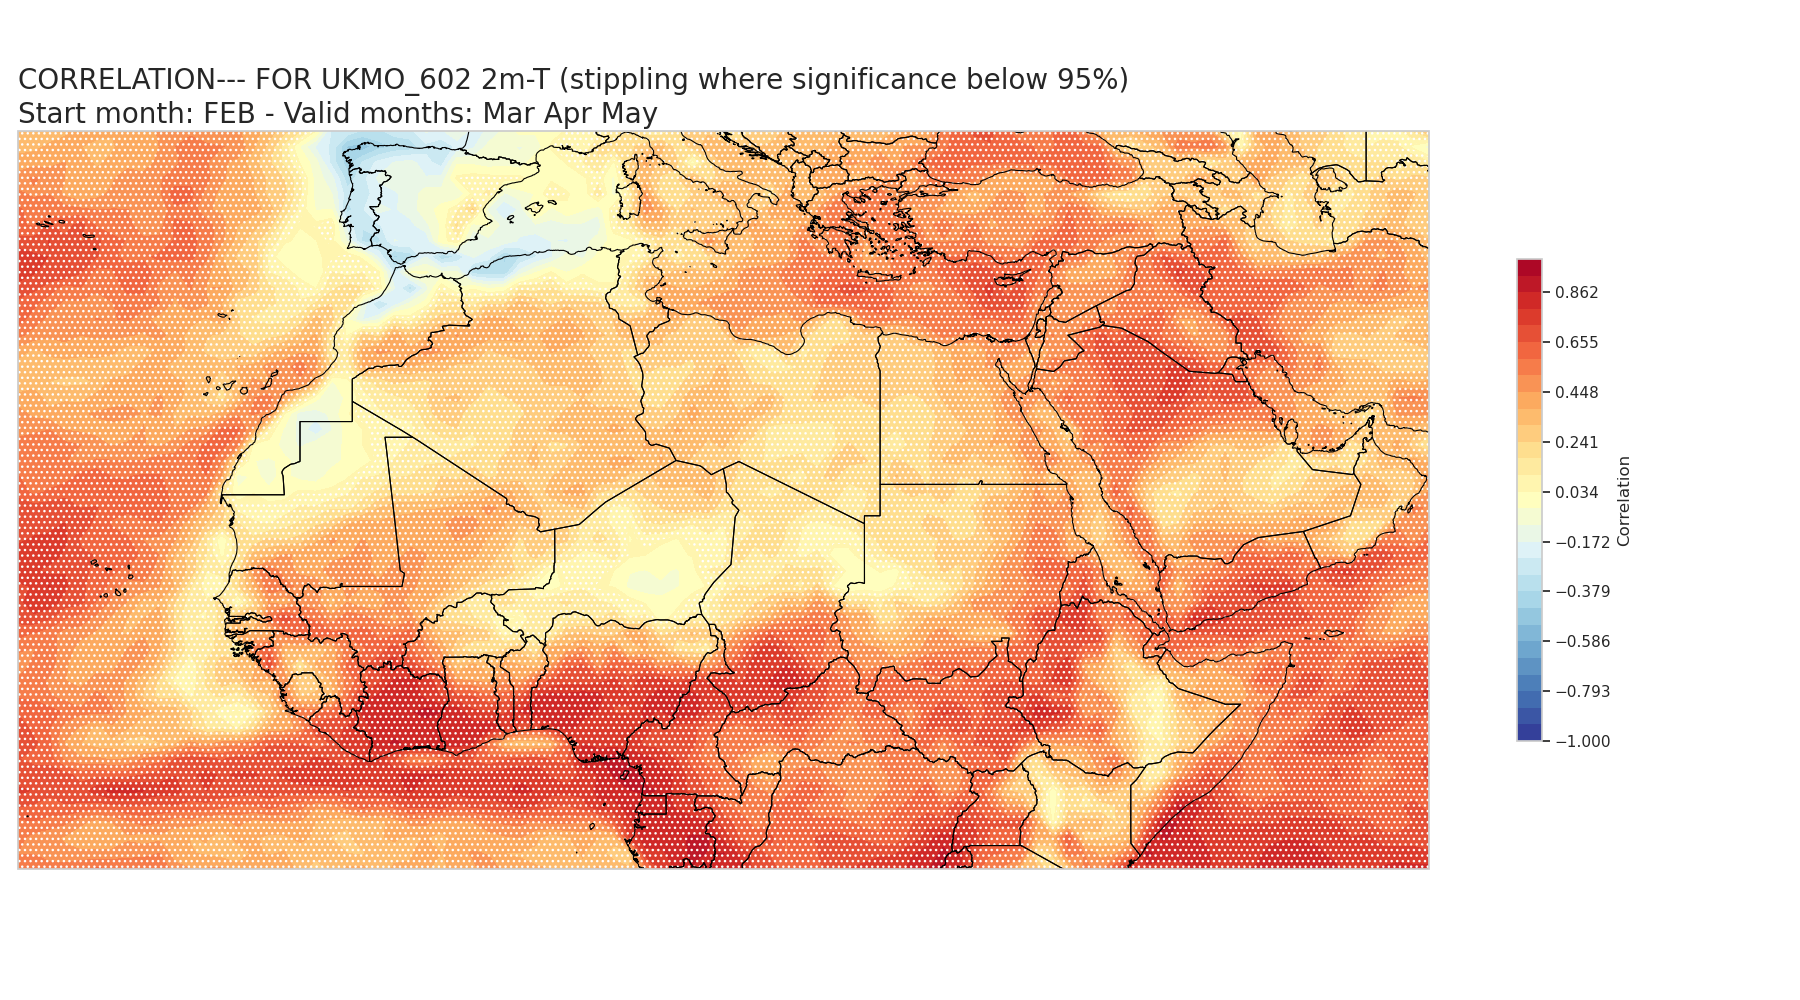
\includegraphics[scale=0.3]{titlepage.png} 
    \end{figure}

    % Author and Supervisors
    \Large
    \textbf{Authors:} \\
    Nohayla BERRAHMOUCH, Mohamed EL-BADRI \\
    \textit{Hassania School of Public Works}

    \vspace{0.5cm}
    \textbf{Supervised by:} \\
    Wafae BADII (Direction Generale de la Meteorologie, Morocco)\\ Nicholas Savage (Met Office, Exeter, UK) \\ Idriss BARI (Direction Generale de la Meteorologie, Morocco)

    \Large
    \textbf{Hassania School of Public Works}

    \vspace{0.8cm}

    % Date (optional)
    \Large
    \textbf{2024}

    \vspace{0.31cm}

    
\end{titlepage}


% Table of contents and section formatting
\tableofcontents
\newpage


\section*{Acknowledgments}
Most importantly, we would like to give special thanks and deep appreciation to \textbf{Mrs. Waafae Badi}. Her endless support and sagacious counsel encouraged us to withstand various difficulties under the project. The feedback, knowledge, and open manner with which she was willing to work to help us face some of the barriers encountered are praised with satisfaction. Because of her guidance pushing us to work harder, our journey would not have been as productive.\\

Nicholas Savage’s time was funded via the WISER MENA project. The Weather and Climate Information Services (WISER) Programme is funded with UK International Development from the UK government and led by the Met Office in the UK. This work has been partially supported by UK International Development from the UK government; however, the views expressed do not necessarily reflect the UK government’s official policies. \\ 


Many thanks to \textbf{Mr. Nicholas Savage} and his great team at the UK Met Office; it was because of their immense generosity and knowledge with considerable resource selection that our work was truly able to traverse actual lines. New doors opened for us that day; discussions and interactions with them broadened our horizons for climate modeling and energized the project itself. Their dedication and commitment toward climate science raised the spirits and empowered the aspiration to reach high.\\

Finally, we wish to extend our considerable gratitude to \textbf{Mr. Bari}, whose position was the supervisor providing guidance and assessing progress on the project. His intelligent suggestions, moderate-though-motivating feedback, and consistent willingness to provide practical assistance during our time of troubles enhanced the preparation of this work. We really appreciated his outstanding, constant support to promote progress and guarantee quality throughout the lifetime of this project.



In this context, we would like to extend our profound gratitude to all those whose fingers contributed to this project. Their cooperation and guidance have ensured that some aspects of the path were easier and enriched the process. But above all, this project is not the work, so it concludes, of the supposedly successful; it is, instead, a conundrum expedition of all those who believed in us. 
\newpage

\section*{Preface}
The MENA seasonal forecasting models have undergone both probabilistic and deterministic evaluations. This research study is regarded as the pioneering work and the first of its kind in this area which helps in situational context improvement in seasonal forecasting models. Given the alarming rate of increase in the impacts caused by extreme climatic events including severe droughts, and extreme heat and other climate sensitive issues in the MENA region, this work is a key contribution towards alleviating these issues=
\\

Due to climatic extremes in the MENA region, agriculture, human livelihood, and natural resources are heavily affected. Consequently, it has become almost necessary to have forecasts of seasons that are credible so as to characterize the impacts, or to enhance preparedness. Although seasonal forecasting models have been widely researched and practiced in many parts of the world, their use in MENA countries’ local level remains scarce. This gap is resolved in this study, providing new knowledge and tools for climate scientists working in the region.\\

In this work, we intend to broaden the knowledge fabric of climate change science by focusing on the climate change and variability vulnerability of the MENA region. The results obtained not only improve the comprehension of the dynamics of the local climate, but also lays a framework for specific approach to be employed for adaptation strategies.\\

We are immensely grateful to every individual or organization who has helped support this project and guided us through uncharted territory in the spectrum of MENA climate predictions.\\
\newpage
\section*{Overview and Rationale of the Study}
The last couple of decades have witnessed a surge in demand for seasonal climate forecasting. Global advancements in space science and technology have lead to the better anticipation of climate seasons up to a thorugh range of 3-12 months. This is crucial for effective planning in major industries like agriculture or energy management, amongst others. These advancements breed an increased dependence on seasonal forecasting and in turn create a higher demand for accurate forecasting mechanisms. Therefore two central methodologies have witnessed prominence – deterministic and probabilistic methods. A hindsight understanding of these mechanisms is imperative, as they are useful for evaluating and understanding the shortcomings and effectiveness of different models employed in forecasting seasonal amps.\\

Probabilistic forecasts take one step forward, do not try to predict an ideal scenario and present different potential outcomes, each with a defined probability. Efforts, though different, instruct towards the same ends; meeting a specific operational/strategic need. Lorenz’s butterfly effect presents the case for one such endeavor- it shows how a non-linear system’s response can drastically alter depending on the initial conditions. Such chaos is especially present in weather and climate systems where even the slightest details can have large ramifications over longer periods.\\

The study on the other hand tries to develop such relationships that integrate conceptual developments in seasonal forecasting efforts with applicable methods.
\newpage

\section{Introduction}
\subsection{Context}
\subsubsection{Overview of Climate Modeling and Seasonal Forecasting}
Climate modeling is the process of using mathematical representations of the Earth’s atmosphere, oceans, land surface, and ice systems to simulate and predict climate dynamics. These models are based on fundamental physical principles, such as the conservation of mass, energy, and momentum, and are implemented through numerical methods that solve complex equations governing the interactions between these systems.\footnote{McGuffie, K. and Henderson-Sellers, A., 2014. A Climate Modelling Primer. \url{https://doi.org/10.1002/9781118687853}} Climate models range from global circulation models (GCMs), which simulate large-scale atmospheric and oceanic processes, to regional climate models (RCMs), which provide localized projections by incorporating finer-scale topographic and land-use details.\footnote{Flato et al., 2013. Evaluation of Climate Models. IPCC AR5 Chapter 9. \url{https://www.ipcc.ch/report/ar5/wg1/chapter-9-evaluation-of-climate-models/}} Seasonal forecasting, a subset of climate modeling, refers to the prediction of climate conditions, such as temperature and precipitation, over a period of one to six months. These forecasts rely on initial conditions (e.g., sea surface temperatures, soil moisture) and slowly varying components of the climate system, such as oceanic or atmospheric anomalies like the El Niño-Southern Oscillation (ENSO).\footnote{Doblas-Reyes, F. J., García-Serrano, J., Lienert, F., Biescas, A. P., \& Rodrigues, L. R., 2013. Seasonal climate predictability and forecasting: Status and prospects. \url{https://doi.org/10.1038/ngeo1714}} The basic principle behind seasonal forecasting is to leverage these slowly varying components, which have a predictable influence on regional weather patterns, using ensemble simulations to quantify uncertainties and provide probabilistic predictions.\footnote{Palmer, T. N., \& Anderson, D. L., 1994. The prospects for seasonal forecasting—a review paper. \url{https://doi.org/10.1256/smsqj.50402}}  

Seasonal forecasts play a crucial role in decision-making and planning across various sectors, including agriculture, water management, and climate risk mitigation. These forecasts provide early warnings of high-impact climate scenarios, enabling proactive decisions that result in financial savings, risk reduction, and optimized resource use. For instance, in agriculture, they assist farmers in selecting appropriate crops and determining optimal planting times based on anticipated water availability, thereby mitigating risks associated with droughts or excessive rainfall.\footnote{Werner, M. and Linés, C., 2024. Seasonal forecasts to support cropping decisions. \url{https://doi.org/10.5194/egusphere-egu24-13436}} Seasonal forecasts also support pre-harvest strategies, such as hedging decisions, which help shield farmers from price volatility, although their adoption is often hindered by perceptions of inaccuracy and complexity.\footnote{Hunt et al., 2020. Seasonal Forecast Based Preharvest Hedging. \url{https://doi.org/10.22004/AG.ECON.309761}} In water management, seasonal forecasts are vital for mitigating drought impacts, particularly in semi-arid regions, by enabling improved reservoir operations and efficient water allocation to reduce losses.\footnote{Portele et al., 2021. Seasonal forecasts offer economic benefits for hydrological decision-making. \url{https://doi.org/10.1038/s41598-021-89564-y}} Additionally, these forecasts, when linked to hydrological models, improve predictions of water balance and inform critical decisions regarding water storage and distribution, despite occasional discrepancies between predicted and desired variables.\footnote{MacLeod et al., 2023. Translating seasonal climate forecasts into water balance forecasts. \url{https://doi.org/10.1371/journal.pclm.0000138}} Seasonal forecasts are increasingly applied in climate risk management, where they help predict extreme weather events, providing decision-makers with tools to minimize societal and economic damages.\footnote{Castino et al., 2023. Towards seasonal prediction of extreme temperature indices. \url{https://doi.org/10.5194/ems2023-590}} For example, accurate predictions of heatwaves or floods allow authorities to implement adaptive measures, reducing infrastructure damage and safeguarding public health. In economic sectors such as energy and water management, tailored seasonal forecasts enhance decision-making efficiency by aligning forecasts with user needs, thereby optimizing outcomes.\footnote{Goodess et al., 2022. The Value-Add of Tailored Seasonal Forecast Information. \url{https://doi.org/10.3390/cli10100152}} Despite their significant potential, the effectiveness of seasonal forecasts depends on their accuracy, relevance to user needs, and ease of use. Improved communication, stakeholder training, and efforts to bridge the gap between forecast complexity and user understanding are essential to maximize their utility.



\subsubsection{Importance of Seasonal Climate Forecasts in MENA}
Seasonal climate forecasts are critically important across the MENA region, where high temperatures, low water availability, and vulnerability to climate variability create substantial challenges for sustainable development. Forecasts provide early warnings of droughts, heatwaves, and other extreme weather events, enabling decision-makers to implement proactive measures to mitigate impacts on water resources, agriculture, and infrastructure.\footnote{Dunn et al., 2020. The changing climate of MENA. \url{https://pubs.giss.nasa.gov/abs/gu00200u.html}} In agriculture, these forecasts help farmers optimize crop selection and planting schedules, reducing the risks of crop failure in this water-scarce region.\footnote{Werner, M., and Linés, C., 2024. Seasonal forecasts to support cropping decisions. \url{https://doi.org/10.5194/egusphere-egu24-13436}} In the water sector, seasonal forecasts guide reservoir management by predicting rainfall variability, improving water storage strategies, and ensuring more equitable water distribution.\footnote{Portele et al., 2021. Seasonal forecasts for hydrological decision-making. \url{https://doi.org/10.1038/s41598-021-89564-y}} With increasing climate risks, these forecasts also support disaster risk management by allowing governments to prepare for extreme events, such as heatwaves and floods, which are becoming more frequent in the region due to climate change.\footnote{Castino et al., 2023. Towards seasonal prediction of extreme temperature indices. \url{https://doi.org/10.5194/ems2023-590}} Moreover, the economic benefits of using seasonal forecasts are significant. By enabling energy companies to anticipate peak demand periods driven by heatwaves, and by helping municipalities optimize water usage during droughts, these forecasts provide cost savings and efficiency gains.\footnote{Goodess et al., 2022. Value-Add of tailored seasonal forecast information. \url{https://doi.org/10.3390/cli10100152}} However, challenges persist in ensuring the accuracy and usability of these forecasts. The arid and semi-arid nature of much of the MENA region, coupled with complex interactions between regional climate drivers, makes it difficult to provide highly localized forecasts.\footnote{Latif et al., 2011. ENSO predictability and regional climate impacts. \url{https://doi.org/10.1175/2010JCLI3405.1}} Addressing these challenges through improved modeling techniques and stakeholder engagement will be critical to maximizing the value of seasonal forecasts in the MENA region, ensuring better preparedness and resilience against a changing climate.


\subsection{Objectives of the Work}
The primary objective of this work is to evaluate the effectiveness of climate models, focusing specifically on their performance in predicting key climate variables such as temperature, precipitation. This evaluation incorporates both deterministic and probabilistic approaches to identify the most skillful models and their suitability for practical applications.

\subsubsection{Specific aims  of evaluating deterministic and probabilistic models.
}
The evaluation of deterministic and probabilistic models is essential for understanding their unique strengths, limitations, and potential applications in diverse fields. Deterministic models, which generate a single, precise outcome based on initial conditions, are widely used when exactness and reproducibility are critical, such as in engineering and physical simulations.\footnote{McGuffie, K., and Henderson-Sellers, A., 2014. *A Climate Modelling Primer*. Wiley. \url{https://doi.org/10.1002/9781118687870}} Their evaluation focuses on assessing accuracy and reliability under specific conditions, providing clarity in cause-and-effect relationships. In contrast, probabilistic models incorporate uncertainty by assigning probabilities to various potential outcomes, enabling the representation of real-world complexities and variability.\footnote{Palmer, T., and Hagedorn, R., 2006. *Predictability of Weather and Climate*. Cambridge University Press. \url{https://doi.org/10.1017/CBO9780511617652}} These models are particularly beneficial for strategic planning and risk management, where understanding a range of possible scenarios is crucial. The evaluation of both types of models includes conducting sensitivity analyses to determine how changes in input variables affect outcomes, which helps in identifying key drivers of uncertainty and improving model performance.\footnote{Seneviratne, S.I., et al., 2021. *Metrics for climate model evaluation: A review*. Nature Communications. \url{https://doi.org/10.1038/s43247-021-00094-x}} Additionally, risk assessment is a vital component, with deterministic approaches offering straightforward estimations for defined scenarios, while probabilistic approaches address uncertainties by simulating a spectrum of possible outcomes.\footnote{PreventionWeb, 2021. *Deterministic and Probabilistic Risk*. \url{https://www.preventionweb.net/understanding-disaster-risk/key-concepts/deterministic-probabilistic-risk}} These evaluations also aim to support decision-making processes by identifying which type of model is more appropriate for specific contexts—deterministic models for precise predictions and probabilistic models for flexible planning under uncertainty.\footnote{Goodess, C.M., et al., 2022. *The Value-Add of Tailored Seasonal Forecast Information for Industry Decision Making*. Climate. \url{https://doi.org/10.3390/cli10100152}} Finally, probabilistic models are often recognized for their adaptability in dynamic environments, as they can incorporate new data and adjust probability distributions to reflect evolving conditions, making them indispensable for complex systems where deterministic models may fall short.\footnote{Latif, M., and Keenlyside, N., 2011. *El Niño/Southern Oscillation Predictability*. Journal of Climate. \url{https://doi.org/10.1175/2010JCLI3405.1}} Together, the evaluation of deterministic and probabilistic models provides invaluable insights into their suitability for addressing specific challenges, supporting informed decision-making, and advancing model development.

\subsubsection{Description of Content}

This report is designed to provide a comprehensive analysis of climate model evaluation, focusing on both deterministic and probabilistic approaches. The structure of the report follows a logical progression, starting with an introduction to the fundamental concepts behind climate models. The first section lays the groundwork for understanding the key differences between deterministic and probabilistic models, describing how each approach is used to simulate climate systems and predict future outcomes. The methodology chapter follows, detailing the specific techniques employed to assess the models. This includes the use of both deterministic and probabilistic metrics such as Root Mean Square Error (RMSE), Anomaly Correlation Coefficient (ACC), and Brier Score, which are critical for evaluating the models' accuracy and performance in predicting climate variables like temperature and precipitation.

Next, the report moves on to the results and analysis, where the performance of the selected models is presented and compared. This section highlights the models' strengths and weaknesses, providing insight into how well they predict climate patterns across various geographical regions and time periods. Special attention is given to the models' skill in forecasting extreme weather events, which are particularly relevant to sectors like agriculture, water resource management, and disaster risk reduction.

The final section of the report provides conclusions and recommendations based on the analysis. This chapter synthesizes the findings, offering practical suggestions for improving the accuracy, usability, and application of climate forecasts. Recommendations also address how future developments in climate modeling can better meet the needs of decision-makers and stakeholders. The report as a whole seeks to contribute valuable insights into the ongoing development of climate prediction systems, aiming to enhance their effectiveness in real-world applications.






  % Include content from nohaila.tex file
\chapter{LITERATURE REVIEW}
\section{Overview of Climate Models}
\subsection{Deterministic Models}
Deterministic models rely on mathematical equations that describe the physical processes of the atmosphere. These models use fixed initial conditions to provide precise predictions, making them suitable for short-term forecasting. However, due to the chaotic nature of atmospheric systems, as demonstrated by Lorenz's theorem, deterministic models are limited in their ability to predict long-term outcomes. Small errors in initial conditions can lead to significant differences in results, reducing their reliability for seasonal or long-term forecasting.\footnote{Lorenz, E. N. (1963). Deterministic Nonperiodic 
Flow. \textit{Journal of the Atmospheric Sciences, 20}(2), 130–141.}

Deterministic climate models operate based on fixed initial conditions and mathematical equations that simulate physical processes in the atmosphere. These models are particularly useful for short-term predictions as they provide precise and singular forecasts. However, deterministic models are significantly limited when forecasting over extended periods. This limitation arises due to the inherent sensitivity of atmospheric systems to initial conditions—a concept known as the \textit{butterfly effect}, introduced by Edward Lorenz in 1963. His research demonstrated that even minute changes in the initial conditions of a system could lead to vastly different outcomes over time, emphasizing the chaotic nature of weather systems.

For seasonal forecasting, deterministic models often fail because minor errors in the initial conditions can amplify, resulting in inaccurate predictions for longer timescales. Despite these challenges, deterministic models are vital for understanding specific phenomena over shorter durations with high spatial and temporal resolution.

\subsection{Probabilistic Models}
Probabilistic models address the limitations of deterministic approaches by incorporating uncertainty into forecasts. Instead of producing a single outcome, these models generate a range of possible scenarios, each with an associated probability, using ensemble simulations or statistical techniques. This makes probabilistic models particularly useful for medium- to long-term forecasts and risk assessment in climate-sensitive sectors such as agriculture, water management, and disaster mitigation.\footnote{World Meteorological Organization (2024). \textit{Guidance on Verification of Operational Seasonal Climate Forecasts}. \url{https://library.wmo.int/records/item/56227-guidance-on-verification-of-operational-seasonal-climate-forecasts}}

The evaluation of probabilistic models relies on metrics that assess their ability to represent uncertainty and provide actionable insights:
\begin{itemize}
    \item \textbf{Reliability:} Measures how well predicted probabilities align with observed frequencies.
    \item \textbf{Resolution:} Assesses the model’s ability to distinguish between different outcomes.
    \item \textbf{Discrimination:} Evaluates the model’s ability to separate events from non-events.\footnote{Rapport de projet 2024–2025, \textit{3rd Year Meteorology Modeling Project}.}
\end{itemize}

Probabilistic models are especially valuable for decision-making under uncertainty, as they provide stakeholders with a clearer understanding of risks and potential scenarios, enabling proactive measures to mitigate impacts.\\

\textbf{Comparison of Deterministic and Probabilistic Models}\\
Deterministic and probabilistic models serve complementary roles in climate modeling and forecasting. Their distinct features and applications are summarized in Table~\ref{tab:comparison_models}.

\begin{table}[h!]
    \centering
    \caption{Comparison of Deterministic and Probabilistic Models}
    \label{tab:comparison_models}
    \begin{tabular}{@{}p{5cm}p{5cm}p{5cm}@{}}
    \toprule
    \textbf{Feature} & \textbf{Deterministic Models} & \textbf{Probabilistic Models} \\
    \midrule
    Predictability & Produces a single fixed outcome based on initial conditions & Generates a range of outcomes with associated probabilities \\
    \addlinespace
    Sensitivity to Initial Conditions & Highly sensitive, leading to reduced accuracy over long timeframes & Less sensitive due to ensemble techniques reducing error amplification \\
    \addlinespace
    Application Domain & Suitable for short-term, high-resolution tasks, e.g., extreme event analysis & Ideal for medium- and long-term decision-making under uncertainty \\
    \addlinespace
    Use of Historical Data & Limited emphasis on historical variability & Extensively relies on historical data for statistical projections \\
    \addlinespace
    Examples & Global Circulation Models (GCMs), Regional Climate Models (RCMs) & Ensemble forecasting, statistical downscaling \\
    \bottomrule
    \end{tabular}
\end{table}

\noindent While deterministic models are preferred for precise and short-term predictions, probabilistic models provide critical insights into the likelihood of various scenarios, making them indispensable for managing climate-related risks.



\section{ STUDIES IN "MENA".}
\subsection{The current and changing climate in MENA}
Much \footnote{\href{https://www.metoffice.gov.uk/binaries/content/assets/metofficegovuk/pdf/business/international/wiser/wiser-mena-scoping-study-external-v2.pdf}{Met Office WISER Report}} of the MENA region is characterised by high temperature and low water availability, a
combination of variables that have the potential to lead towards the environmental
limits/threshold for safe human habitation. This makes the region
particularly vulnerable to climate change and climate variability, as small variations in climate
can easily produce high temperatures or extensive droughts that are harmful to human lives
and livelihoods.\\

Changes in temperature and rainfall patterns have already been observed in the region and
are expected to change further in the near future, especially if global warming exceeds 1.5 to
2 °C above the pre-industrial level. Annual mean temperatures across the MENA region
have increased between 0.3–0.5°C per decade1 over the period 1980–2015 \footnote{\href{https://pubs.giss.nasa.gov/abs/gu00200u.html}{(Gutiérrez et al.,
2021)}}. Since the 1950s, hot and cold extremes have become warmer, the number of cold
days has decreased, and the number of warm days has increased (Dunn et al., 2020). There
has been an increase in heat waves intensity, frequency and duration    \footnote{\href{https://www.nature.com/articles/s41467-020-16970-7}{(Perkins-Kirkpatrick
and Lewis, 2020)}}. Annual mean precipitation shows a high level of spatial variability over the
MENA region. During the period 1980–2015 there have been downward trends in mean
annual precipitation \footnote{\href{https://pubs.giss.nasa.gov/abs/gu00200u.html}{(Gutiérrez et al., 2021)}} . Dry conditions, drought intensity and frequency
has increased in the past over the region \footnote{\href{https://www.nature.com/articles/s43247-021-00094-x}{(Seneviratne et al., 2021).}} 


\begin{figure}[H]
	\centering
	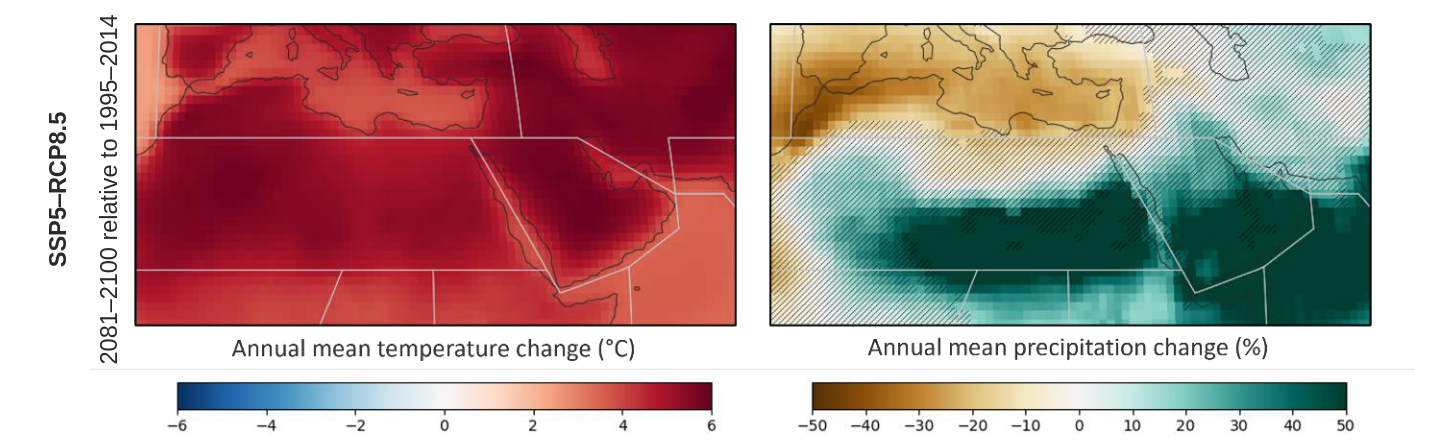
\includegraphics[scale=0.25]{actual_vs_past.png}
	\caption{Projected change in annual mean temperature (left) and annual mean precipitation
(right) between 1995–2014 and 2081–2100 under the SSP5–RCP8.5 scenario based on CMIP6
models (Gutiérrez et al., 2021). Note that precipitation change is given as a percentage: the
large increases projected over Sahara and Arabian deserts equate to only a few millimetres of
additional rainfall.}
\end{figure}



\subsection{Impact-Based Evaluation}
Impact-based forecasting refers to a type of weather or climate forecasting that goes beyond predicting the meteorological parameters (e.g., temperature, rainfall, wind speed) and instead focuses on predicting the potential impacts of those conditions on society, infrastructure, and ecosystems. The goal is to provide actionable insights that help communities and decision-makers prepare for and mitigate the effects of extreme weather and climate events.

\textbf{Evaluation of Seasonal Forecast Models}\\
An impact-based evaluation\footnote{\url{https://agupubs.onlinelibrary.wiley.com/doi/full/10.1029/2024EF004936 }} \footnote{Zahir Nikraftar, Rendani Mbuvha, Mojtaba Sadegh, Willem A. Landman} was conducted as global study on five seasonal forecast models to identify the most effective for extreme precipitation forecasting (focuses on regions which were vulnerable to wildfire and flooding). The models assessed included:
\begin{itemize}
    \item Centro Euro‐Mediterraneo sui Cambiamenti Climatici (CMCC: version 35),
    \item Deutscher Wetterdienst (DWD: version 21),
    \item Environment and Climate Change Canada (ECCC: version 3),
    \item Météo‐France (version 8),
    \item UK Met Office (UK‐Met: version 601).
\end{itemize}

The findings highlighted the \textbf{\textit{UK‐Met} }  and \textbf{\textit{Météo‐France} } models as consistently superior across all four seasons. Meanwhile, the ECCC and CMCC models exhibited strong performance on specific indices and in particular regions, ranking just below the top two models.

\textbf{ROC Scores and Regional Performance}\\
The ROC scores indicate that forecast models perform exceptionally well in tropical and subtropical regions. This result is consistent with our study and can be attributed to the general predictability of oceanic conditions and the influence of climate drivers such as the El Niño-Southern Oscillation (ENSO). The Météo‐France and UK‐Met models exhibited superior performance during the SON and MAM seasons.

However, the prevalence of grids with no discrimination ROC categories is more common in extratropical regions. This can be attributed to:
\begin{itemize}
    \item Lower predictability of extratropical variations,
    \item Model limitations in capturing interactions between tropical and extratropical regions,
    \item Challenges in representing land surface processes (De Andrade et al., 2019).
\end{itemize}
The CMCC, DWD, and ECCC models often fail to detect extreme events in many extratropical areas, underscoring the stronger performance of the UK‐Met and Météo‐France models in these scenarios.

\textbf{Percent Bias Analysis}\\
The analysis of Percent Bias across four seasons demonstrates a consistent underestimation by forecast models for most extreme wet precipitation indices. Key observations include:
\begin{itemize}
    \item Forecast models underestimate extreme wet precipitation indices while overestimating light precipitation.
    \item Models perform better in capturing the intensity and magnitude of extreme events (e.g., highest daily and multi-day rainfall) compared to the frequency of wet or dry days.
\end{itemize}

In tropical and subtropical regions, models like \textbf{\textit{UK‐Met}}  and \textbf{\textit{Météo‐France} } exhibit strong performance due to their ability to capture large-scale climate patterns. In contrast, extratropical regions show higher biases, reflecting challenges in modeling complex interactions and seasonal variations.

\textbf{Global Model Comparison}\\
The \textbf{\textit{UK‐Met}} model consistently demonstrates lower biases and stronger performance globally compared to the \textbf{\textit{Météo‐France} }  model, highlighting its effectiveness in representing climate patterns. However, all models show limitations in accurately modeling persistent extreme wet and dry periods, particularly in extratropical areas.


\subsection{SYSTEM 7 FRANCE}

seasonal forecasting evaluation has been the subject of numerous studies, with a focus on improving the accuracy and reliability of predictions related to precipitation and other weather parameters. One such study\footnote{https://www.mdpi.com/2674-0494/1/3/16} conducted a probabilistic evaluation of seasonal precipitation re-forecasting from May to November over a period of 23 years (1993–2015). The study utilized the Brier Score (BS) and its decomposition to assess forecast performance, with the aim of providing more reliable and actionable predictions for extreme weather events.

The evaluation was conducted on the operational seasonal forecasting system of Meteo-France, which used 25 ensemble members, perturbed model dynamics, and initial conditions. The system aimed to provide a more detailed probabilistic forecast, in addition to existing deterministic metrics, for both seasonal and intra-seasonal forecasts. The BS was estimated using tercile probabilities and a non-parametric counting estimator, with the GPCP\footnote{Global Precipitation Climatology Project (GPCP)} observation data serving as the reference.

Multiple analyses were performed to evaluate the robustness of the BS score, revealing that spatial distributions of the BS can vary significantly based on the sampling methods, reference data, and ensemble types used. The analysis showed that large errors, especially in the tropical ocean, could be reduced by using hindcast ensemble climatological samples. In particular, errors over the Nino region in the Pacific Ocean could be mitigated using these methods. This highlights the importance of employing various ensemble data sources and reference climatology to enhance the reliability of seasonal forecasts.

A notable finding was the reduction in BS when using ensemble observations, especially in the tropical ocean, suggesting that increasing ensemble size can improve forecast accuracy up to a point. However, this was not the case in all regions, as some areas, such as the tropical Indian Ocean, exhibited high BS even with different analysis methods. The study also found that intra-seasonal analyses showed similar patterns to seasonal hindcasts, but with higher BS due to reduced sample sizes, highlighting the need for higher-resolution models and improved initial conditions.

The study concluded that, despite improvements, probabilistic forecasting still faces challenges, particularly in the tropical regions, where errors fluctuate with lead time. The study emphasized the need for continued development of forecasting methods, particularly in reducing uncertainties in evaluation scores. Future evaluations should expand beyond the BS to include other metrics, such as the forecast skill score and the relative operating characteristic (ROC), to better assess forecast performance and identify system deficiencies.

This study's findings underline the importance of ensemble forecasting and the use of diverse data sources to improve the accuracy of seasonal precipitation forecasts, particularly in tropical regions where predictability remains challenging.


  % Include content from Previous_Studies_MENA.tex file
\section{Methodology}

\subsection{DATA}

The hindcast data used in this study was obtained using the OSOP package\footnote{https://github.com/OSFTools/osop/tree/main/scripts}, a tool developed by the UK Met Office to facilitate the retrieval of climate and meteorological data. The dataset comprises monthly mean seasonal forecasts for temperature over the MENA (Middle East and North Africa) region.


The hindcast data spans the common period 1993–2016 and was downloaded from the Copernicus Climate Change Service (C3S) platform. 


The data was retrieved for the following configurations:
\begin{itemize}
	\item Variable: 2-meter air temperature (t2m).
	\item Forecast Range: Lead times of interest (1–3 months), it includes DJF\footnote{December,January,February}, JJA\footnote{June,July,August}, MAM\footnote{March,April,May}, SON\footnote{September,October,November}
	\item Geographical Area: MENA region.
	\item Temporal Coverage: 1993–2016
	\item the used centers are $UKMO,ECMWF,ECCC_2,ECCC_3,CMCC,Meteo-France_8,DWD$
\end{itemize}


In addition to the hindcast data, this study utilized ERA5 reanalysis data, a state-of-the-art atmospheric reanalysis product produced by the European Centre for Medium-Range Weather Forecasts (ECMWF). 

    

\subsection{Deterministic Evaluation Metrics}

\subsubsection{Spearman rank correlation}

Spearman's correlation is a non-parametric measure of rank correlation 
(statistical dependence between the rankings of two variables). 
It assesses how well the relationship between two variables can be described using a monotonic function (whether linear or not).  

$$r_s=\frac{cov(R[H],R[O])}{\sigma_{R[H]} \cdot \sigma_{R[O]}}$$
where : \\

\begin{itemize}
	\item $r_s : $ spearman rand correlation 
	\item H : the Hindcast.
	\item O : the Observation.
	\item R[x] : the rank of the variable x. 
	\item $\sigma_x : $ standard deviation of the variable x.
\end{itemize}

\begin{figure}[H]
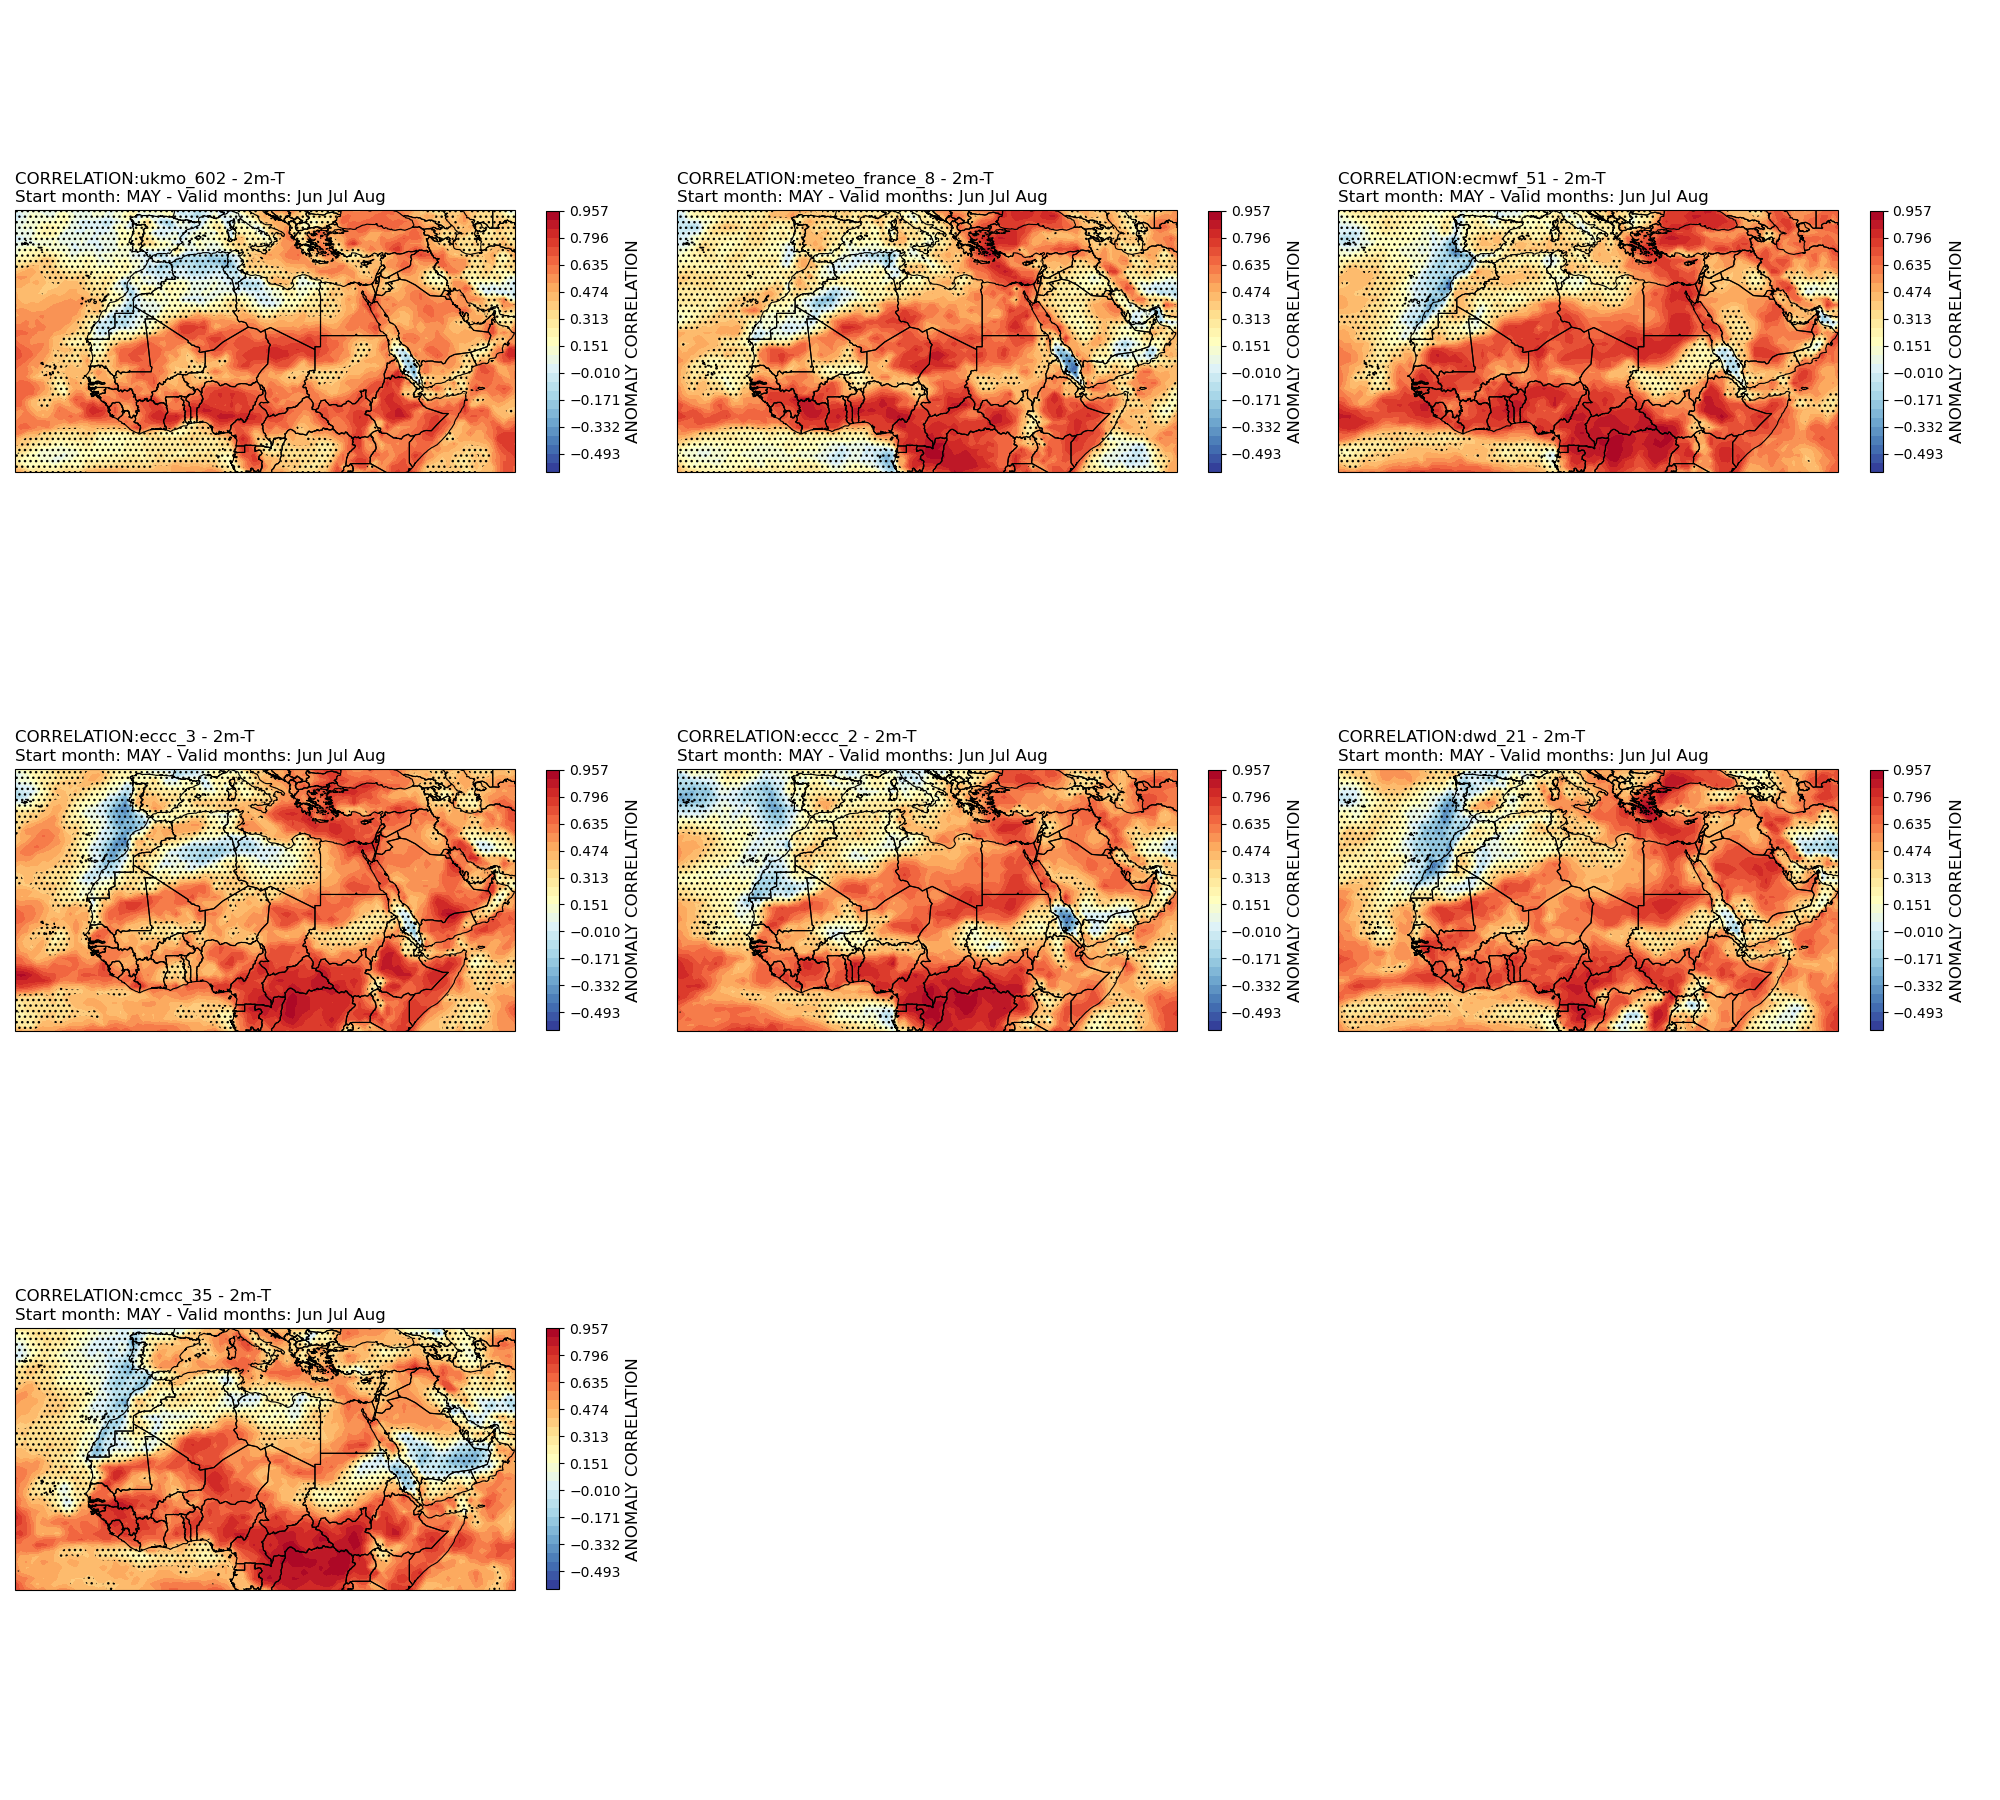
\includegraphics[scale=0.3]{CORR_JJA.png}
\caption{3-months Rolling mean of Spearman Correlation in MENA Region for all centers JJA}
\end{figure}

we can show in the figure above that the best model in term of spearman correlation is the \textbf{ECMWF} center due to the great correlation in all the MENA region especially for   SON\footnote{September,October,November},JJA\footnote{June,July,August} and MAM\footnote{Mars,April,May}.

\begin{figure}[H]
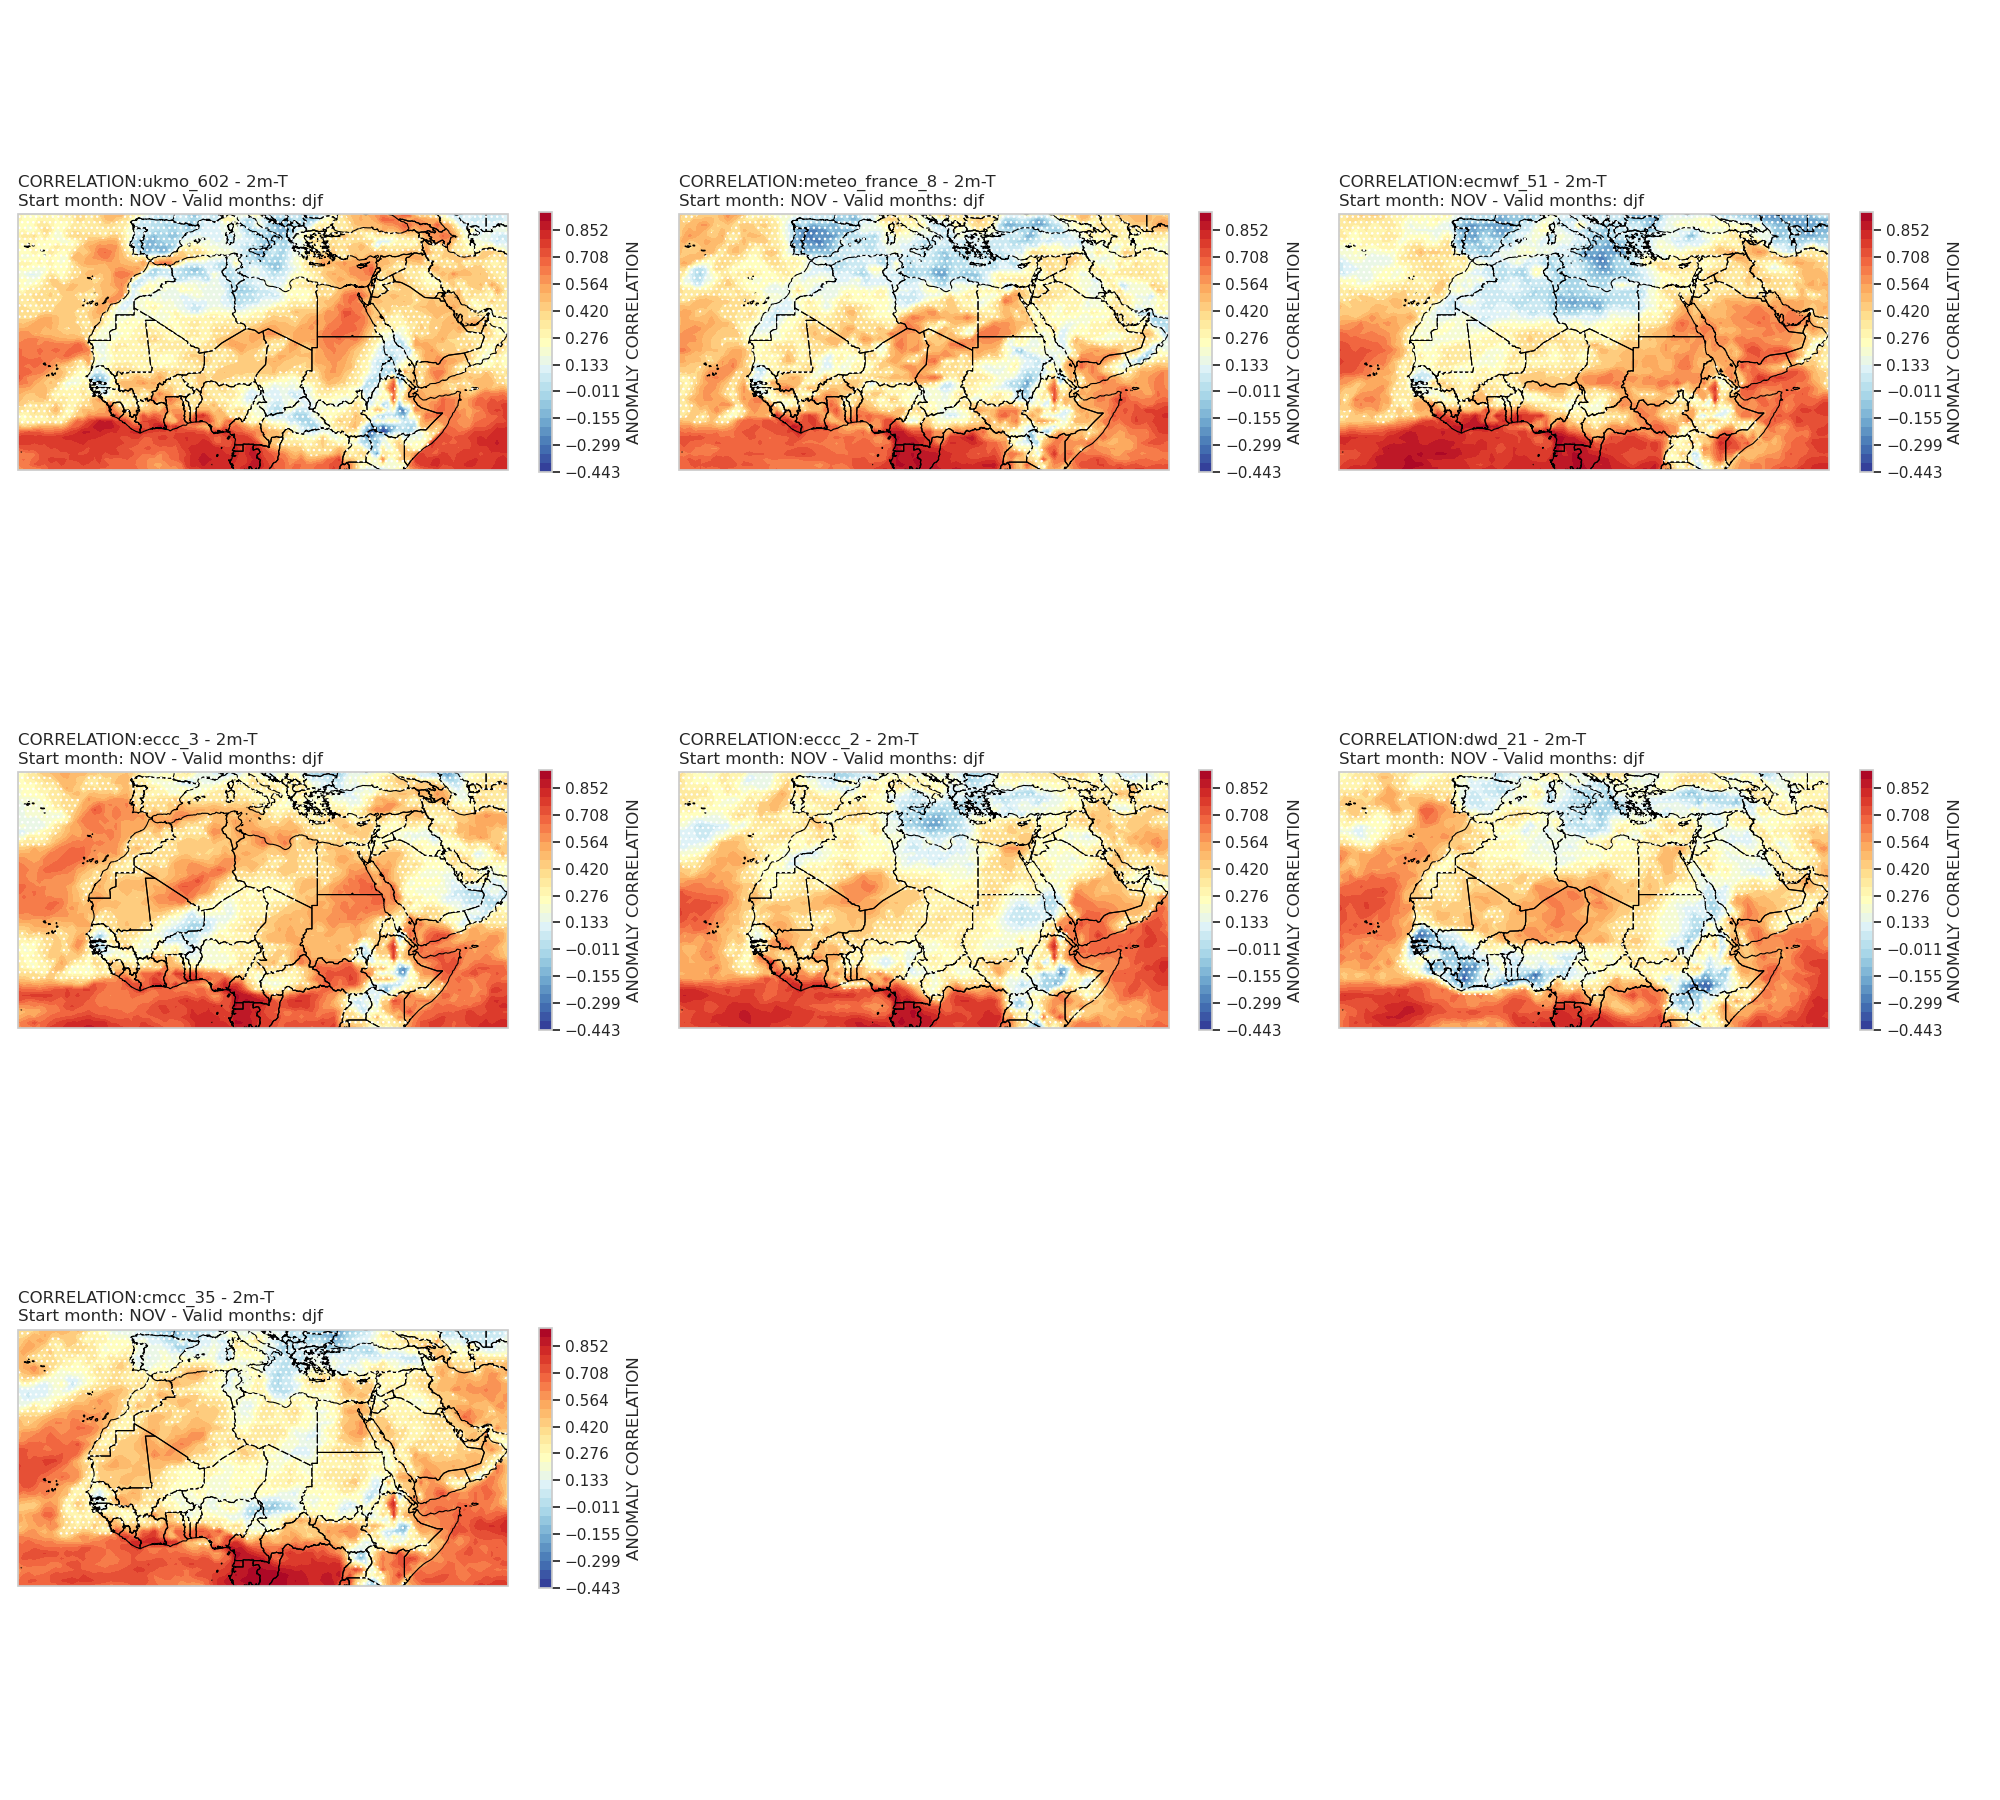
\includegraphics[scale=0.3]{CORR_DJF.png}
\caption{3-months Rolling mean of Spearman Correlation in MENA Region for all centers DJF}
\end{figure}

althought, for DJF\footnote{December,January,February} the ECMWF\footnote{European Centre for Medium-Range Weather Forecasts } , ECCC3\footnote{Environment and Climate Change Canada (ECCC) generation 3}, UKMO\footnote{UK Met Office} and CMCC 35 \footnote{Centro Euro-Mediterraneo sui Cambiamenti Climatici version 3.5} have the same performance.

\begin{figure}[H]
	\centering
	\includegraphics[scale=0.25]{corr_T2M_ PERIOD.png}
	\caption{The Heatmap of correlation for the mena region for every period \textbf{\textit{(1 for perfect Correlation)} }}
\end{figure}




\subsubsection{RMSE}
 
 $RMSE$ measures the average difference between a the hindcast and the observation.
 
$$RMSE=\sqrt{\frac{1}{n} \sum\limits_{i=1}^{n}(H_i -O_i)^2}$$
where :
\begin{itemize}
	\item H : the Hindcast.
	\item O : the observation.
	\item i : the valid time.
\end{itemize}

for the RMSE\footnote{Root Mean Square Error}, the Meteo-France and ECMWF have the best scores for MAM ans SON. Althought, for DJF Météo-France is better, and for JJA ECMWF is the best.

\begin{figure}[H]
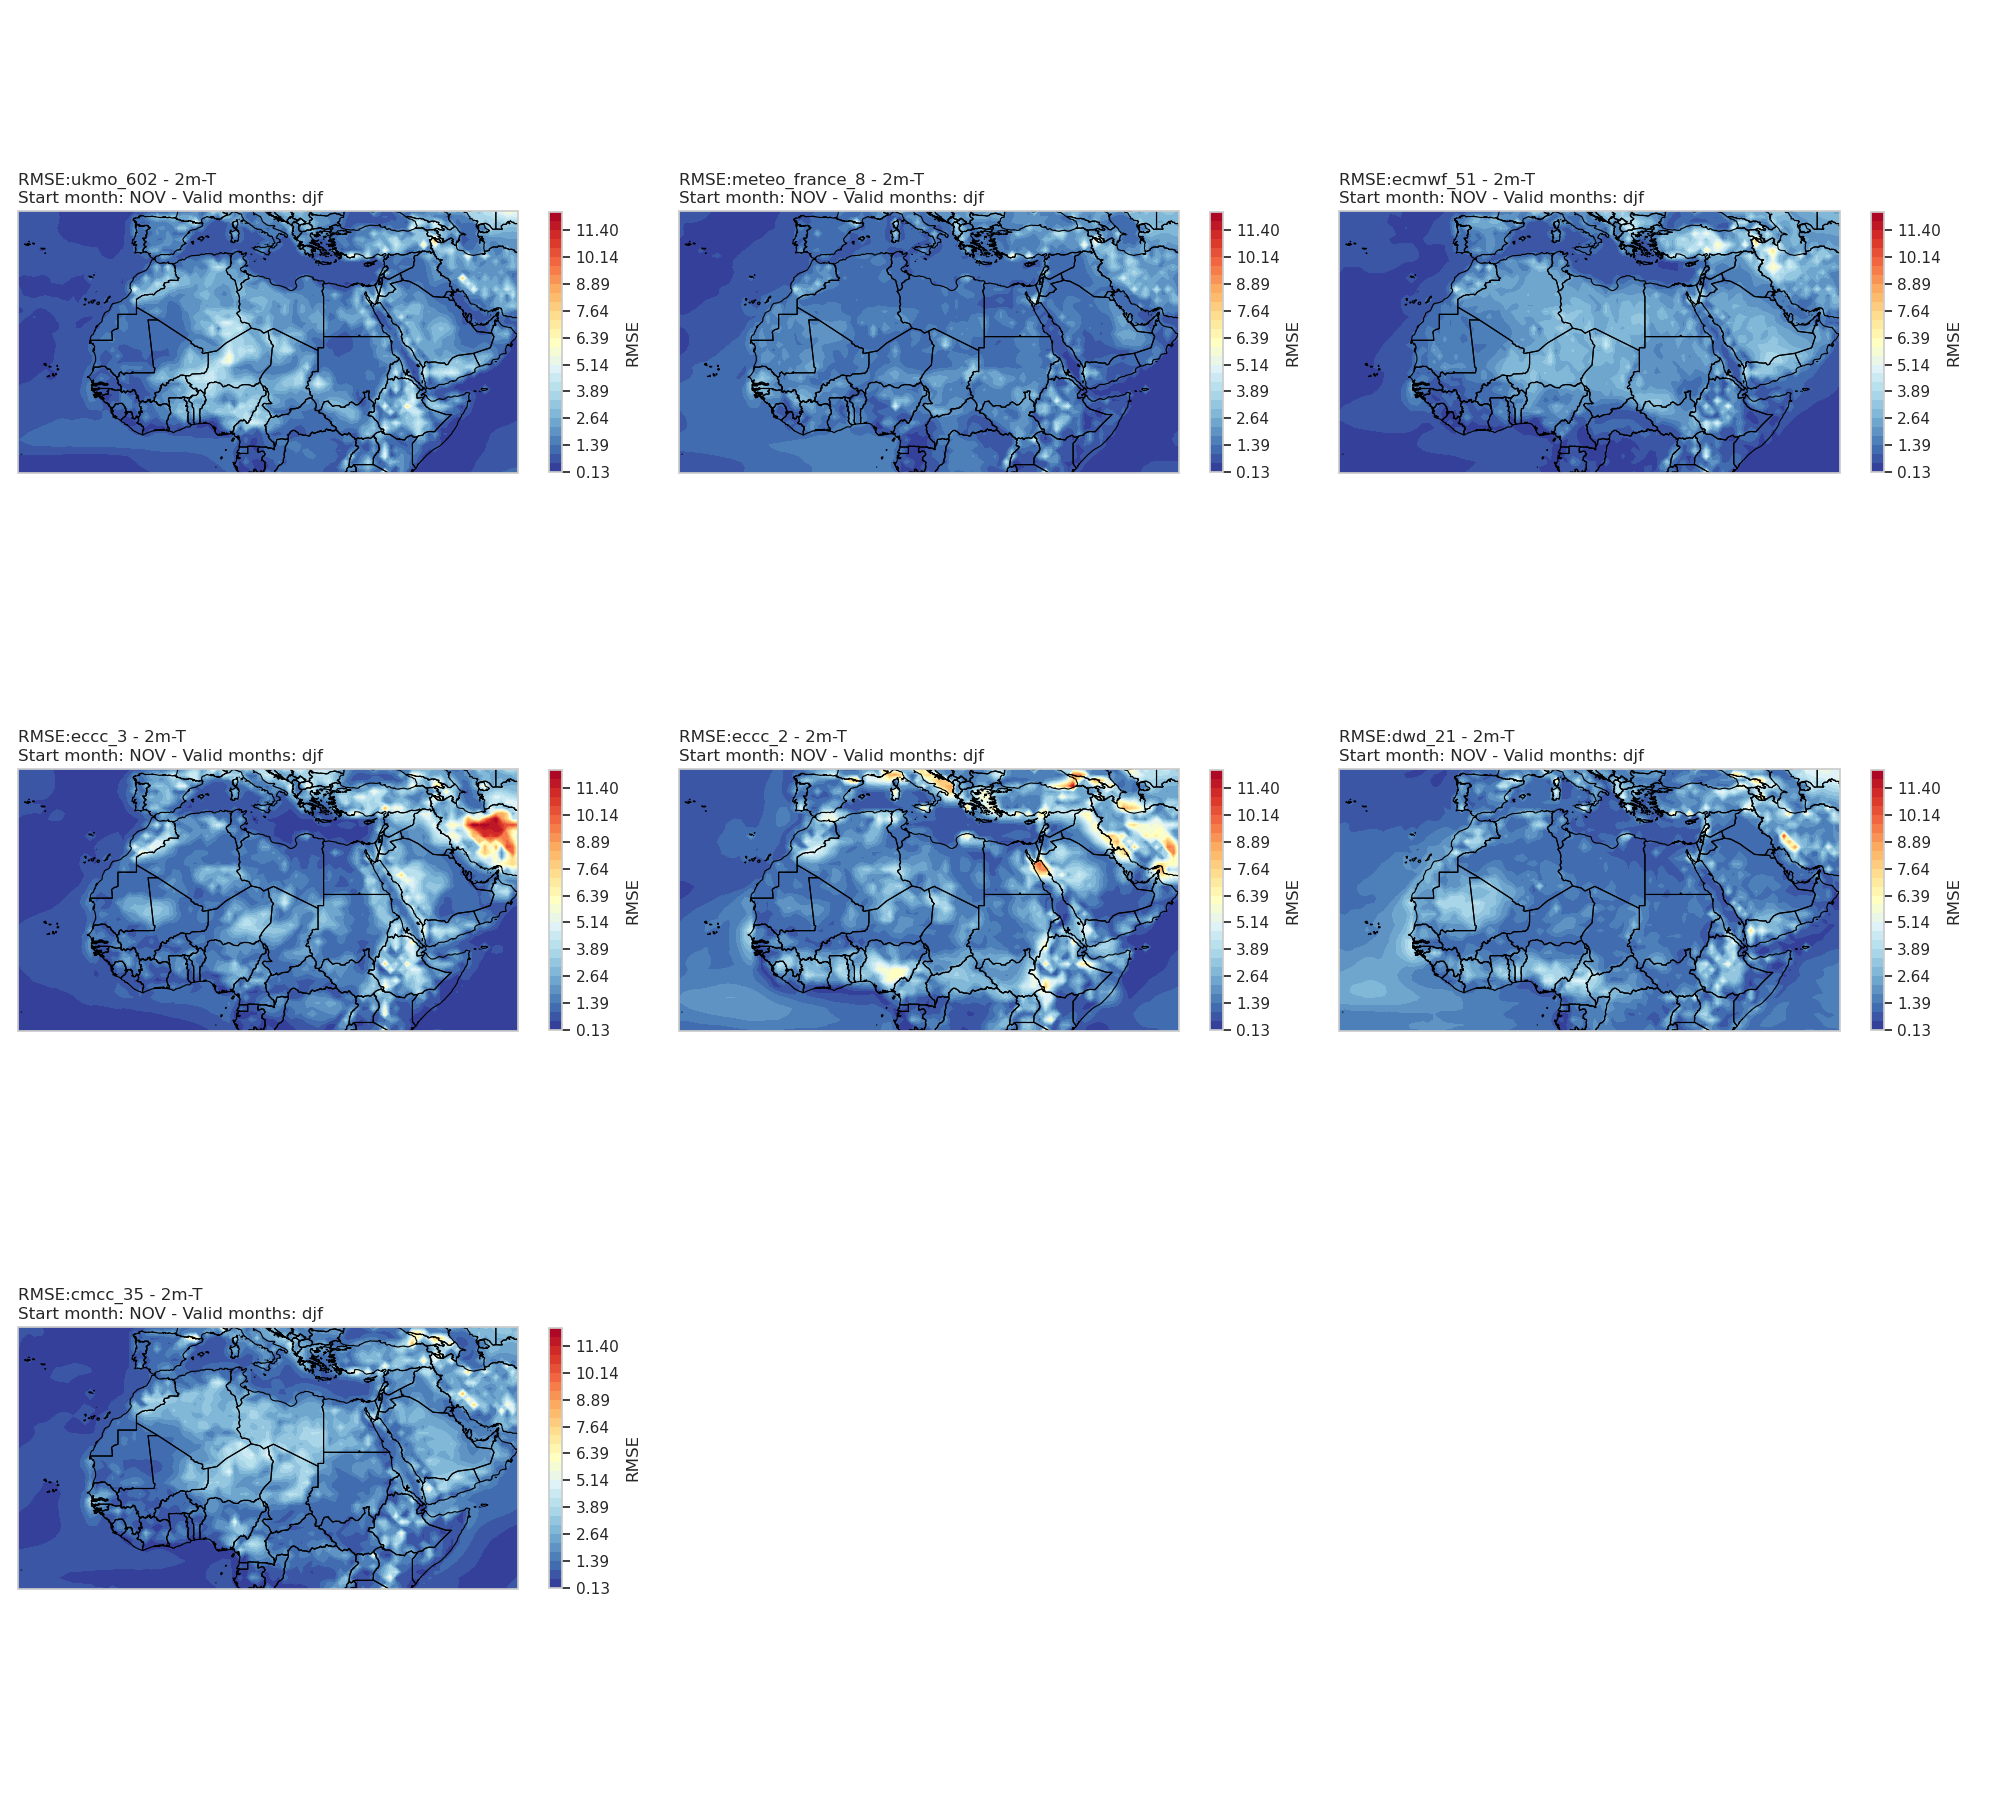
\includegraphics[scale=0.3]{RMSE_DJF.png}
\caption{3-months Rolling mean of RMSE in MENA Region for all centers DJF}
\end{figure}

\begin{figure}[H]
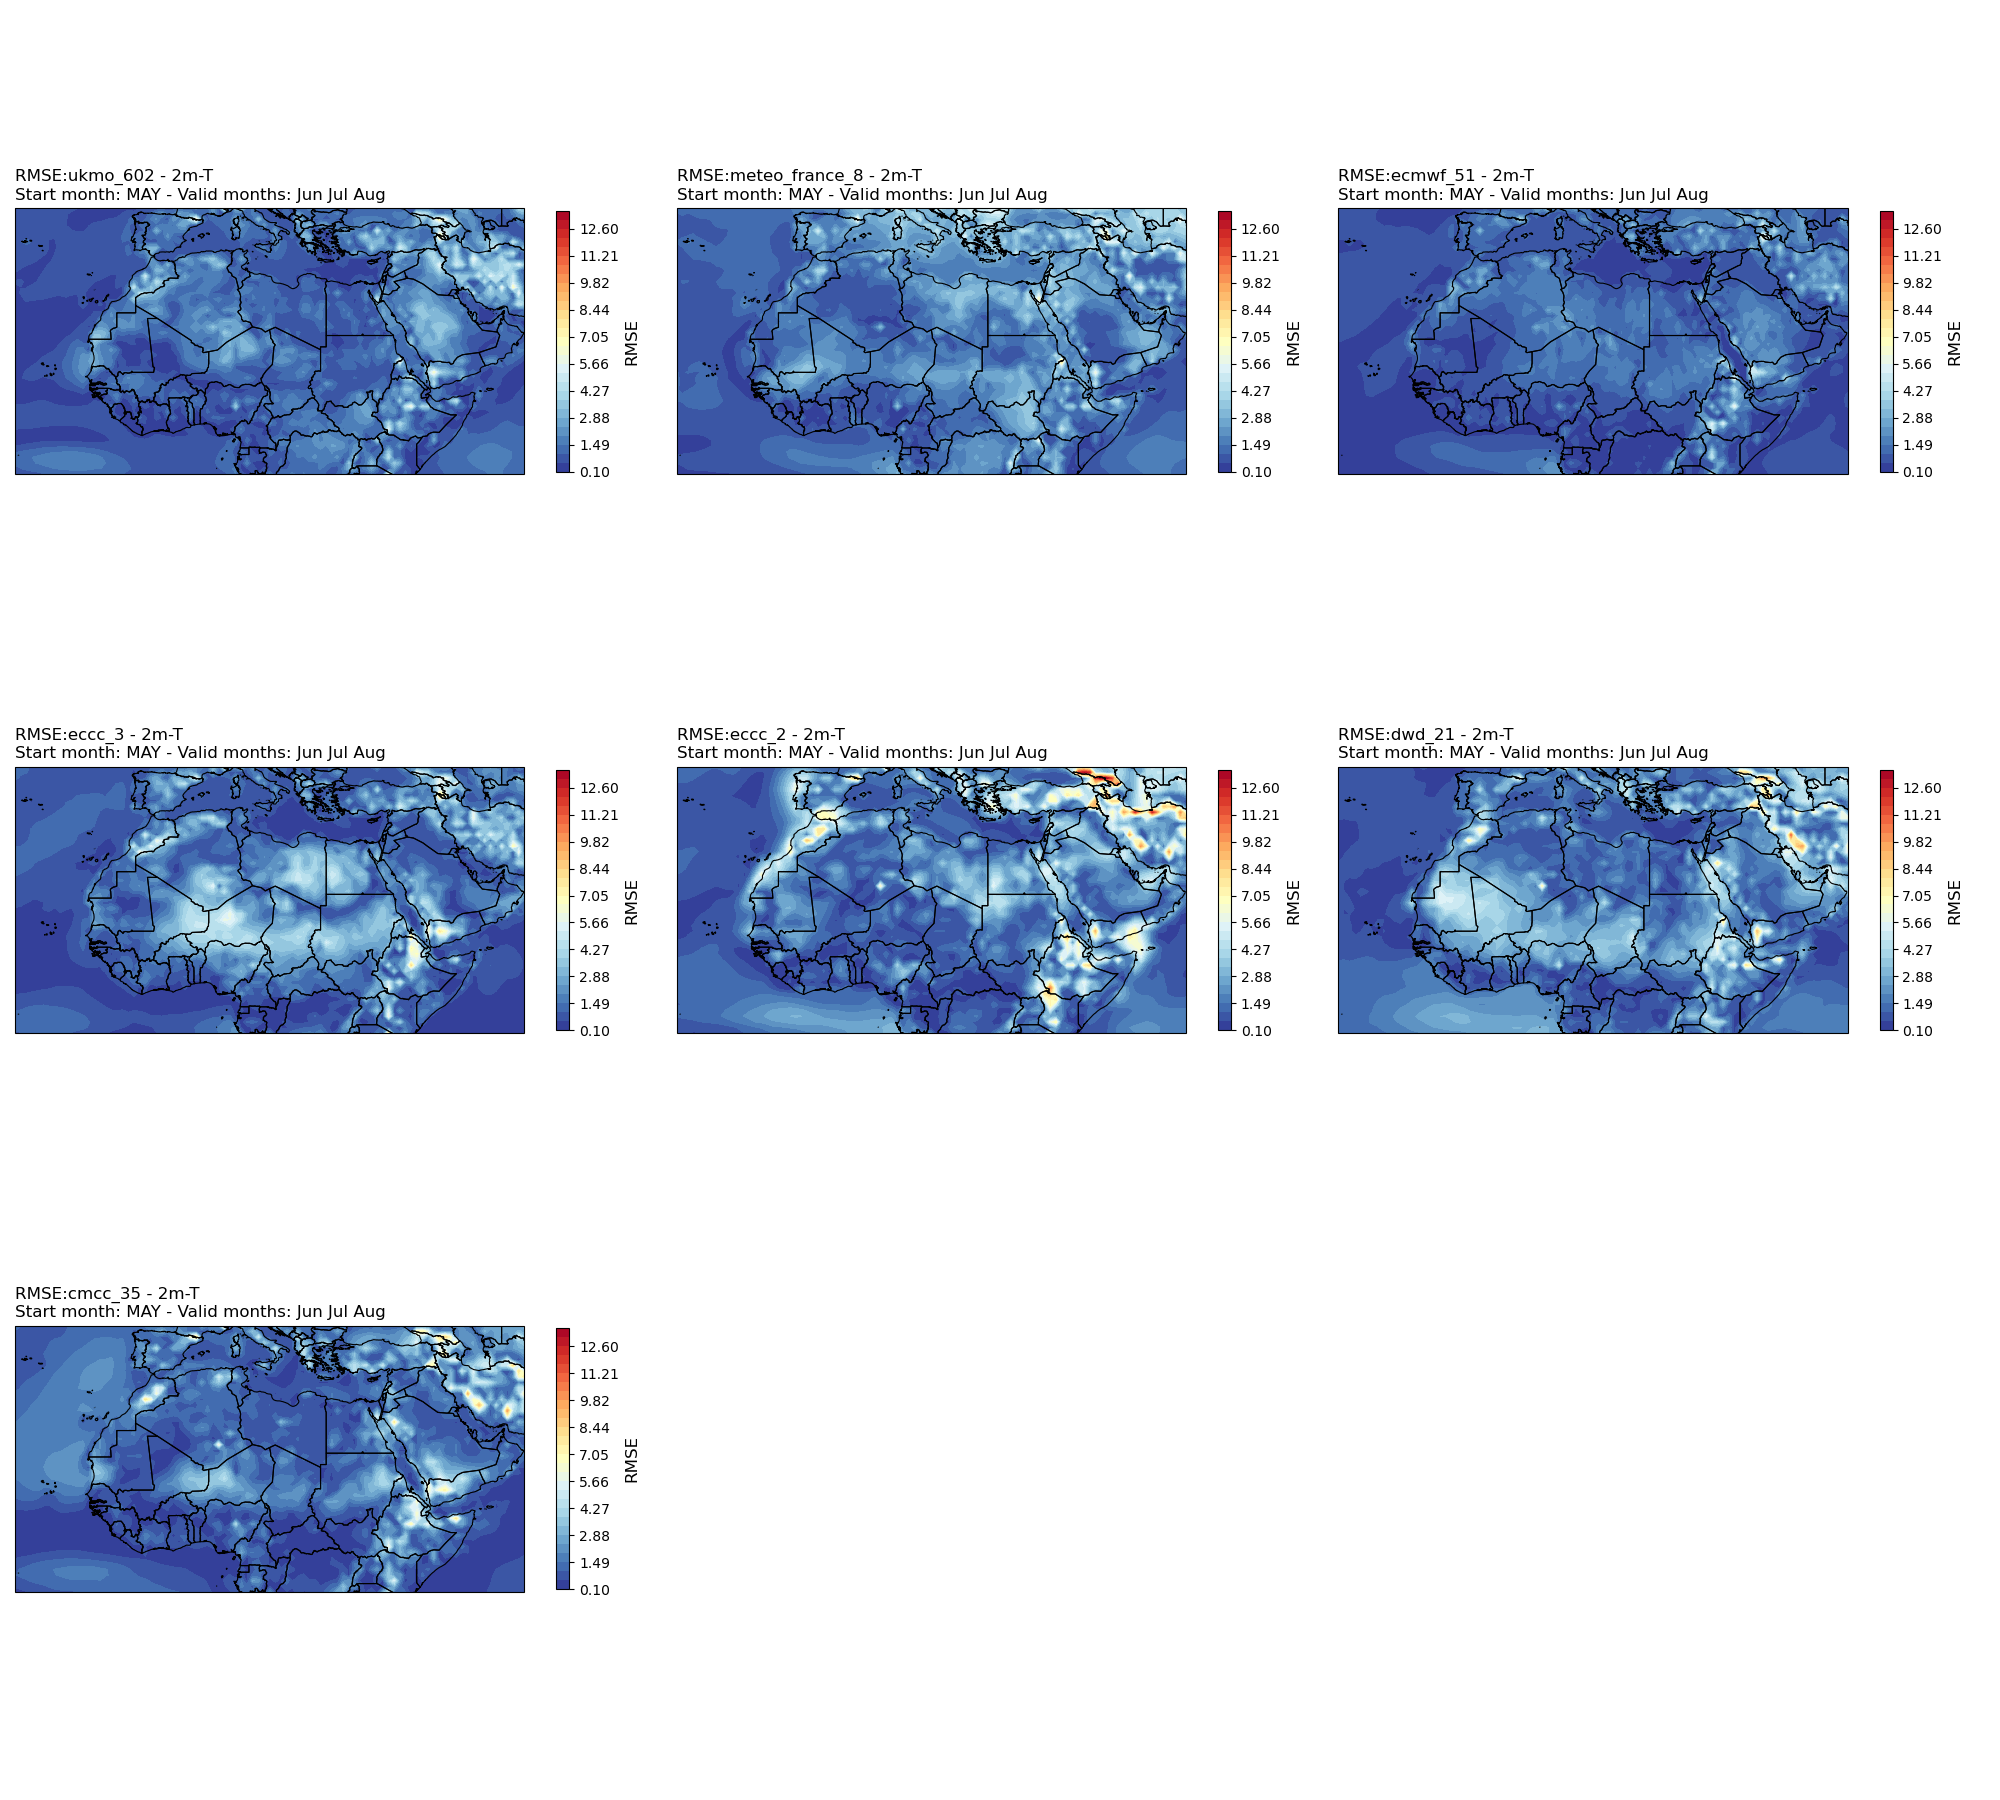
\includegraphics[scale=0.3]{RMSE_JJA.png}
\caption{3-months Rolling mean of RMSE in MENA Region for all centers JJA}
\end{figure}



\begin{figure}[H]
\includegraphics[scale=0.25]{rmse_T2M_ PERIOD.png}
\caption{The Heatmap of RMSE for T2M in the MENA region 
\textbf{\textit{(0 for perfect RMSE)} }}
\end{figure}






\subsubsection{Coefficient of Determination (\( R^2 \))}

The coefficient of determination, \( R^2 \), is a statistical measure used to evaluate the goodness of fit of a model. It indicates the proportion of the variance in the dependent variable that is predictable from the independent variable(s). A value of \( R^2 \) close to 1 suggests that the model explains a large portion of the variance, while a value close to 0 indicates a weak relationship.

\[
R^2 = 1 - \frac{\sum_{i=1}^n (O_i - H_i)^2}{\sum_{i=1}^n (O_i - \bar{O})^2}
\]

where:

\begin{itemize}
	\item \( R^2 \): Coefficient of determination.
	\item \( H_i \): Predicted value (Hindcast).
	\item \( O_i \): Observed value (Observation).
	\item \( \bar{O} \): Mean of the observed values.
	\item \( \sum_{i=1}^n (O_i - H_i)^2 \): Residual sum of squares (unexplained variance).
	\item \( \sum_{i=1}^n (O_i - \bar{O})^2 \): Total sum of squares (total variance).
\end{itemize}

\begin{figure}[H]
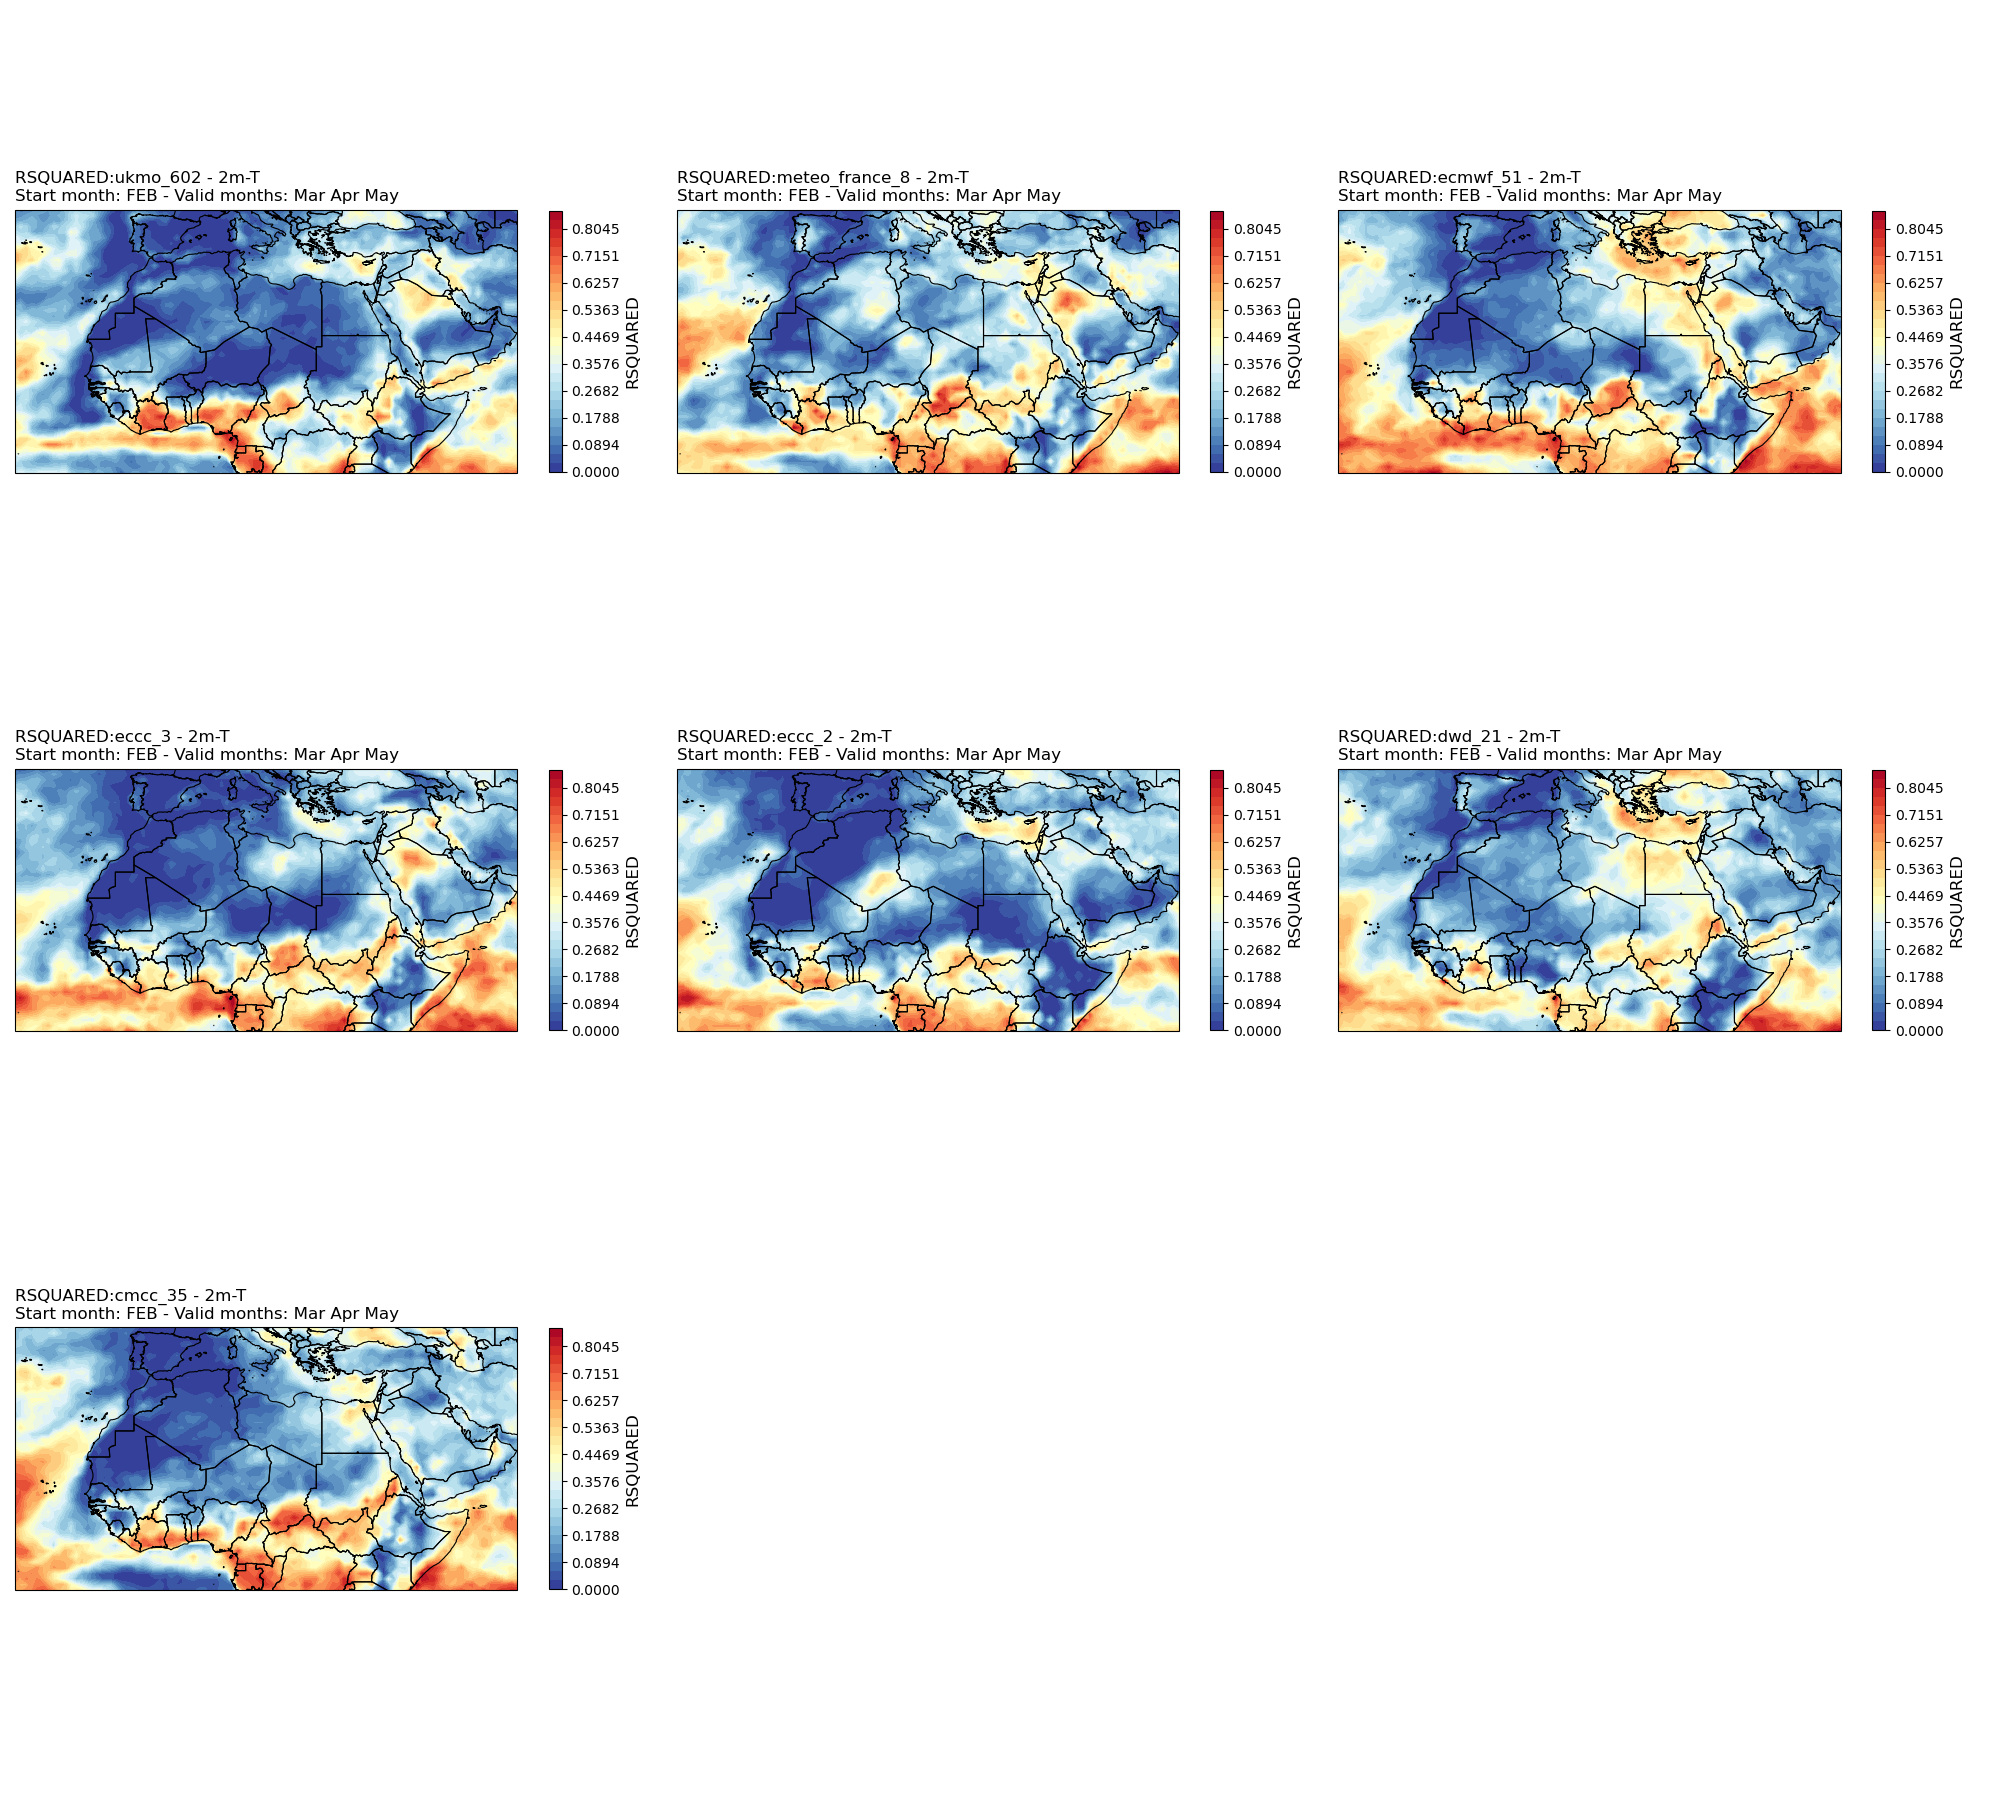
\includegraphics[scale=0.3]{RSQUARED_MAM.png}
\caption{3-months Rolling mean of RSQUARED in MENA Region for all centers MAM}
\end{figure}

we can show in the figure above that the best model in term of R-SQUARED is the \textbf{ECMWF} center for all periods.

\begin{figure}[H]
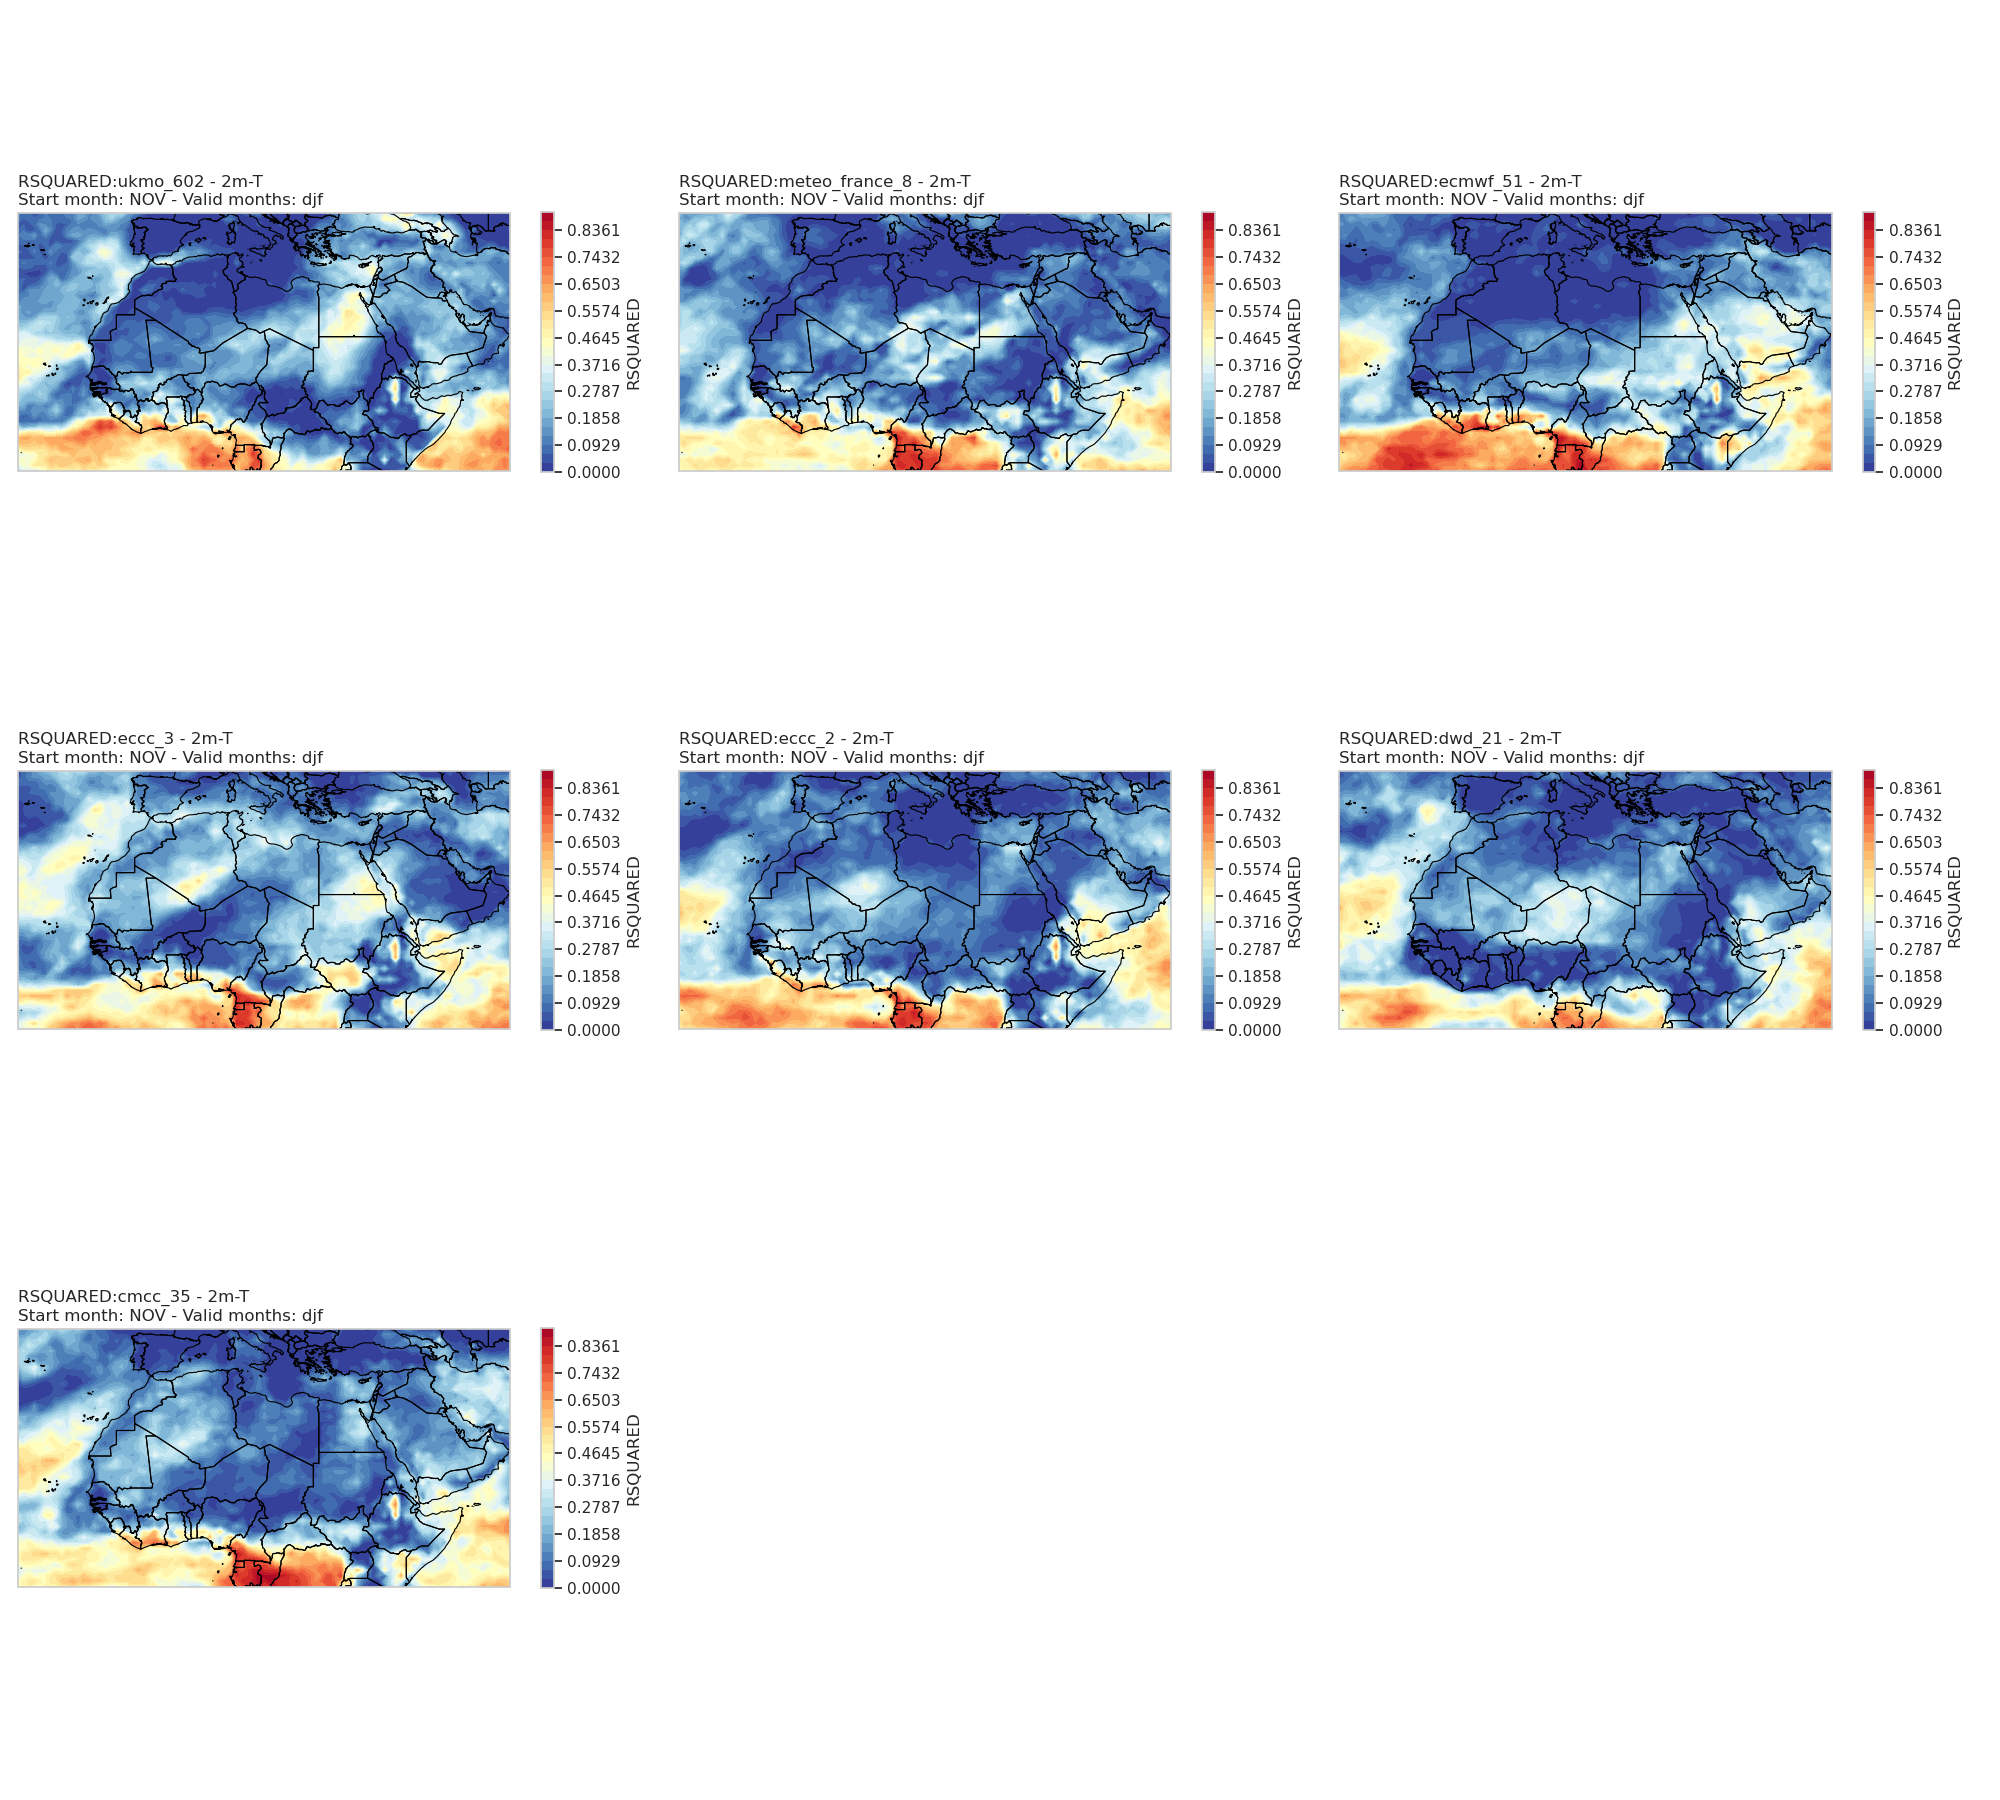
\includegraphics[scale=0.3]{RSQUARED_DJF.png}
\caption{3-months Rolling mean of RSQUARED in MENA Region for all centers DJF}
\end{figure}


\begin{figure}[H]
	\centering
	\includegraphics[scale=0.25]{rsquared_T2M_ PERIOD.png}
	\caption{The Heatmap of rsquared for T2M in the mena region for every period \textbf{\textit{(1 for perfect RSQUARED)} }}

\end{figure}



\subsection{Probabilistic Evaluation Metrics}

\subsubsection{The Brier Score (BS)}
The Brier Score (BS)\footnote{wmo guidance verification} is the mean squared differences between pairs of forecast probabilities p and the binary observations y. N is the total forecast number. It measures the total probability error, considering that the observation is 1 if the event occurs, and 0 if the event does not occur (dichotomous events).

$$BS_j=\frac{1}{N} \sum\limits_{i}^{N} (y_{j,i} - p_{j,i})^2$$

where:
\begin{itemize}
	\item n is the number of forecasts
	\item $y_{j,i} $ is 1 if the $i^th$ observation was in category $j$, and is 0 otherwise.
	\item $p_{j,i}$  is the $i^th$ forecast probability for category $j$.
\end{itemize}
The BS takes values in the range of 0 to 1. \textbf{\textit{Perfect forecasts receive 0}} and less accurate forecasts receive higher scores. Under the condition that x is 0.5 when the observation data is uncertain, the mean squared differences between the forecast probabilities and observation at 0.5 is calculated.


\begin{figure}[H]
    \centering
    \includegraphics[scale=0.25]{bs_T2M_category.png}
    \caption{The Heatmap of Brier Score for each category  . \textbf{\textit{(0 represents perfect BS)}}}
\end{figure}

we see in the figure above that Météo-France, ECMWF,DWD and CMCC35 are the best in Brier Score in the MENA region.





\begin{figure}[H]
    \centering
    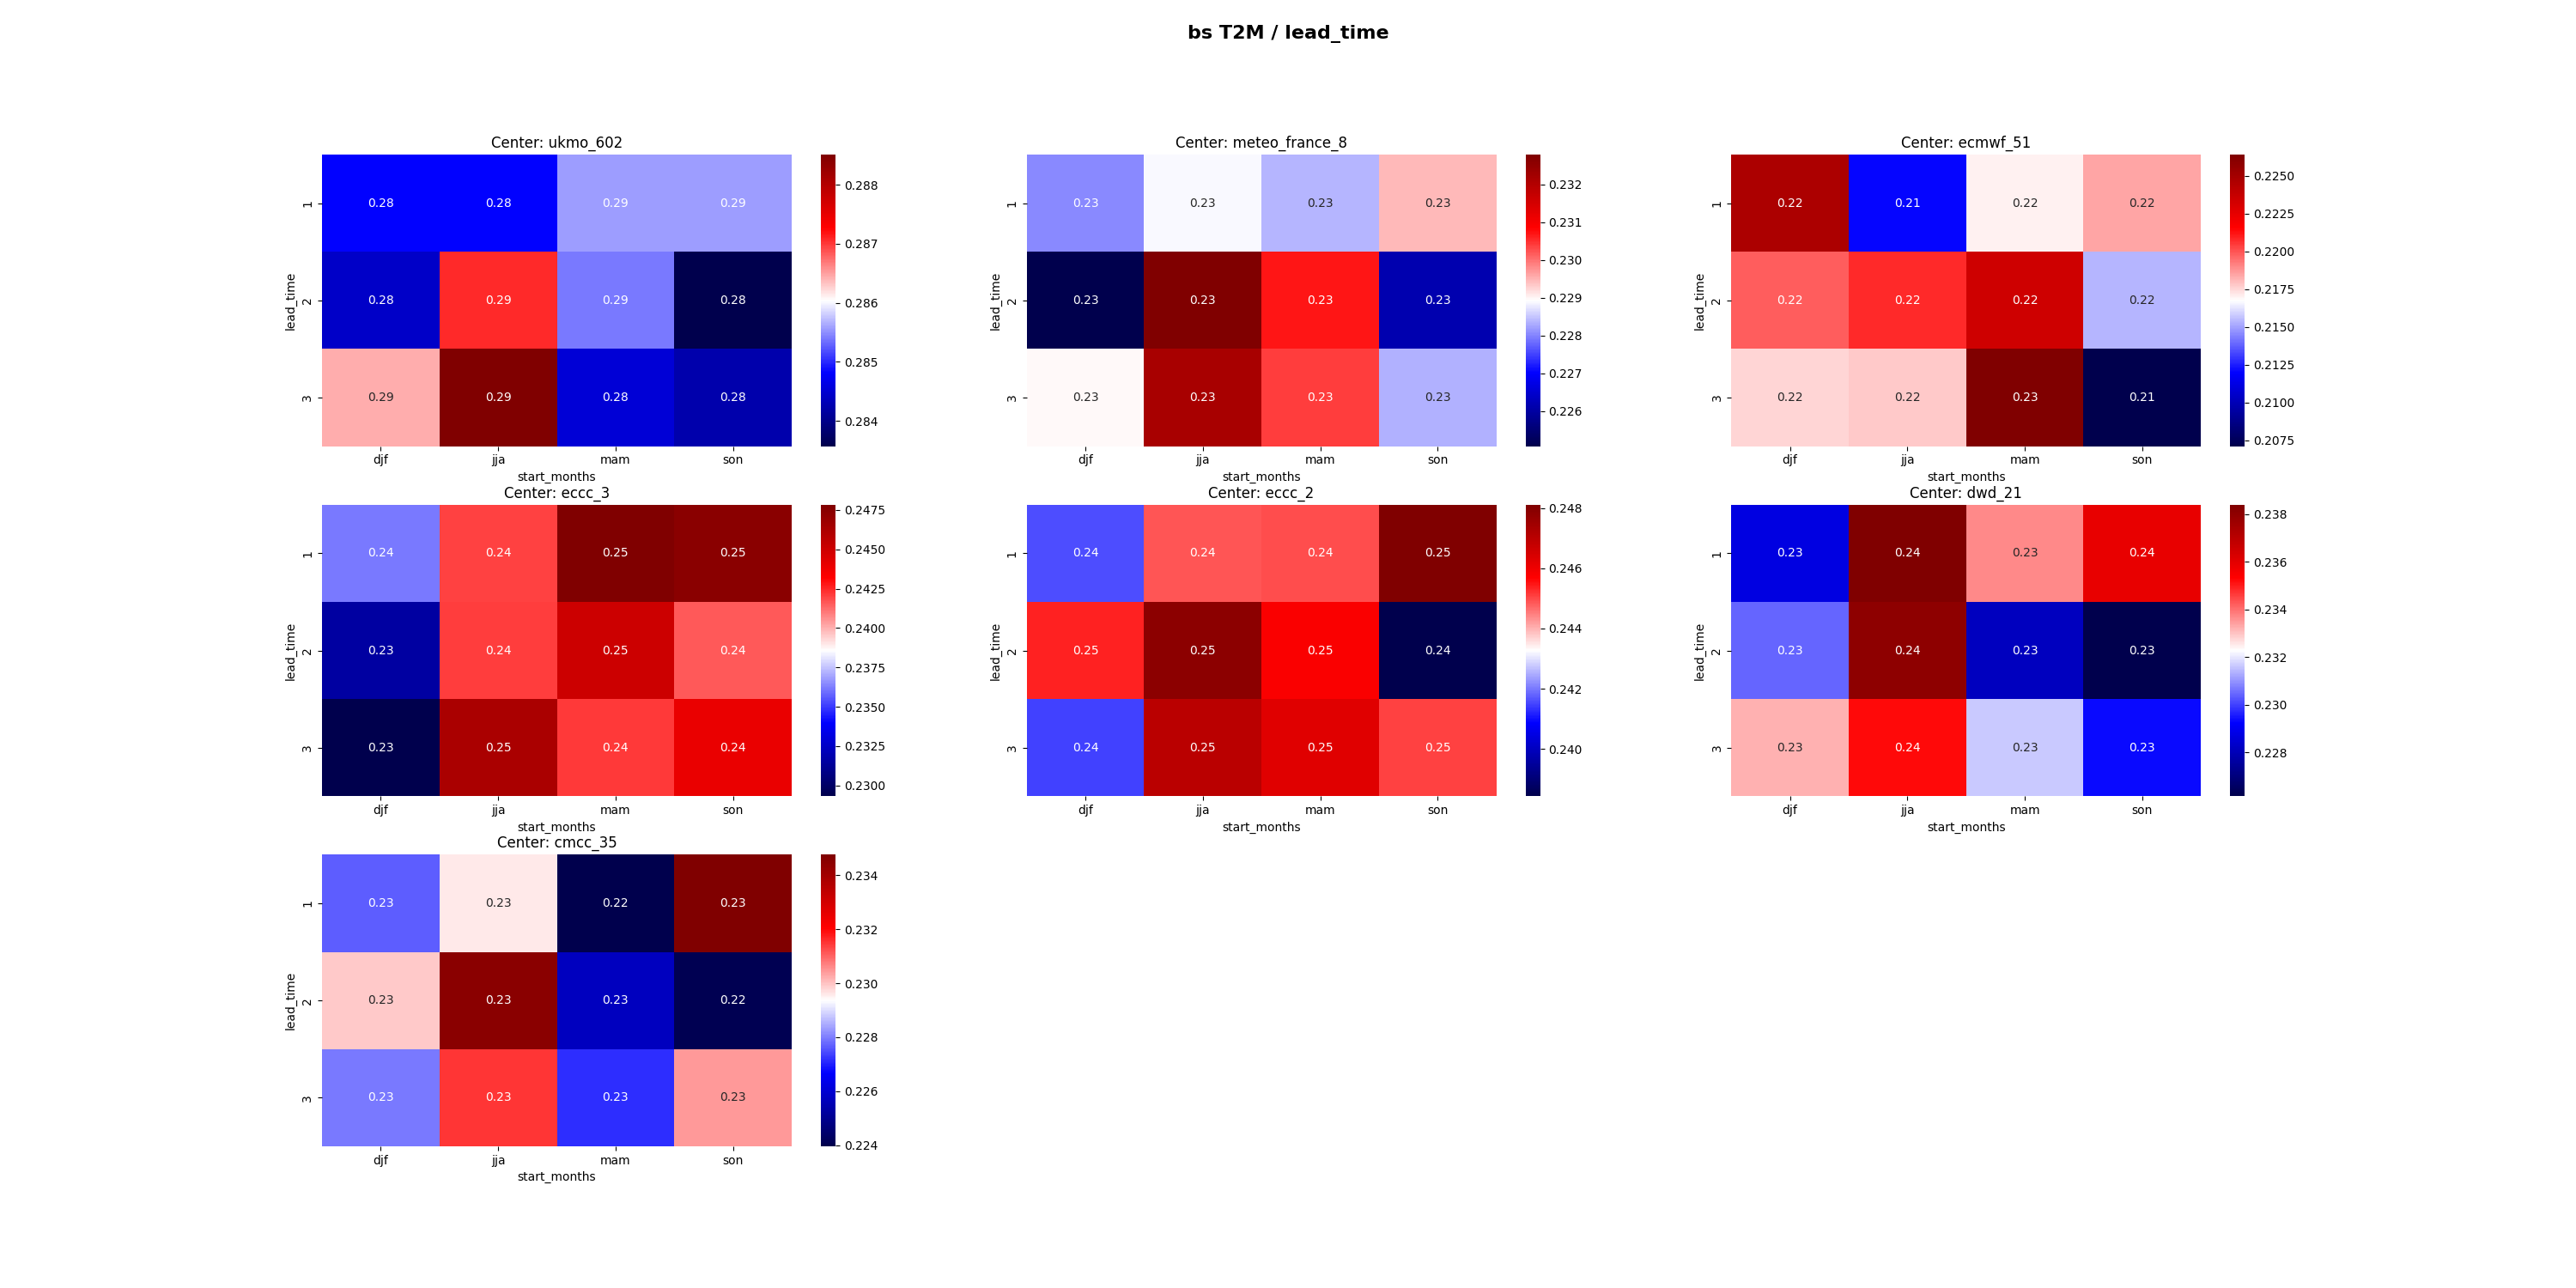
\includegraphics[scale=0.25]{bs_T2M_lead_time.png}
    \caption{The Heatmap of Brier Score for lead-time. \textbf{\textit{(0 represents perfect BS)}}}
\end{figure}
A deep analyze on each tercile category confirms the previous performance.



\subsubsection{Reliability}
the reliability\footnote{wmo guidance verification} measures the degree of correspondence between the forecast probability and the observed frequency for an event or outcome that is being predicted. It summarizes the conditional bias of the forecasts for a given event and is equal to the weighted average of squared differences between the forecast and conditional observed probabilities. If the reliability is 0, the forecast is perfectly reliable. To observe the frequency distribution, the forecast probability, from 0 to 1, is divided into 5 bins (0.1,0.3,0.5,0.7,0.9) to compare to the observed frequency in each of the same bin in this study. 
$$Reliability=\frac{1}{n} \sum\limits_{k=1}^{d} n_k(\bar{p_k}-\bar{y_k})^2$$
where:
\begin{itemize}
	\item $n_k$ is the number of forecasts for the $k_th$ probability value ($\bar{p_k}$)
	\item ($\bar{y_k}$) is the observed relative frequency for that value.
\end{itemize} 

\begin{figure}[H]
    \centering
    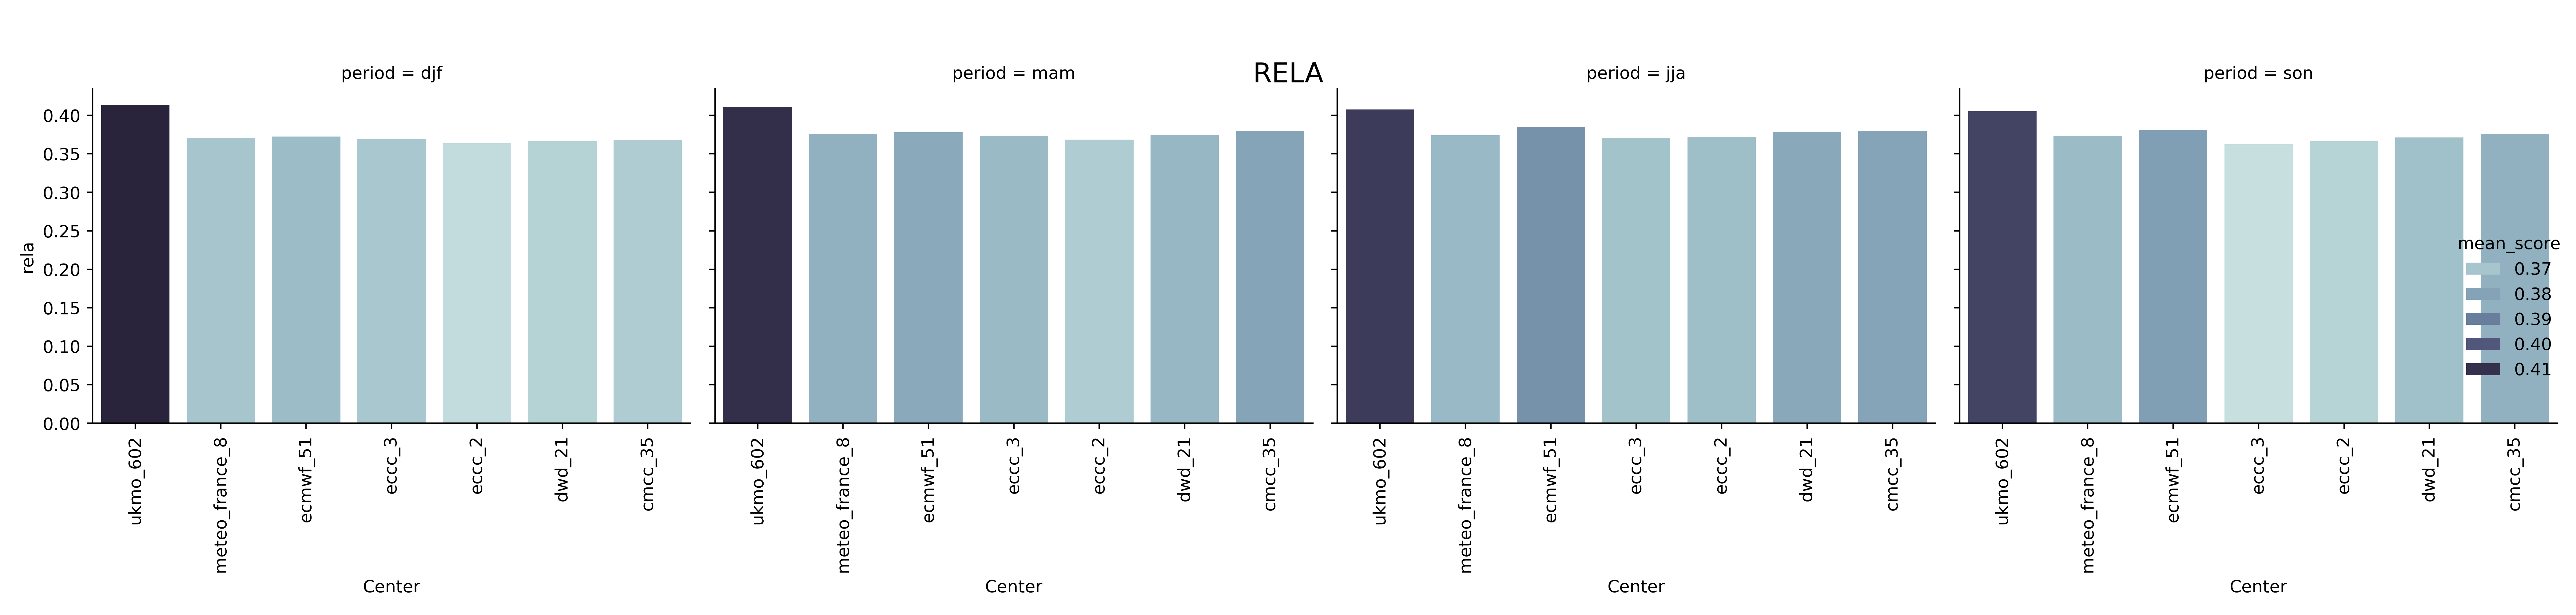
\includegraphics[scale=0.3]{rela_all.png}
    \caption{The Reliability Score  . \textbf{\textit{(0 means perfect Reliability)}}}
\end{figure}

In the figure above, all centers demonstrate similar performance.

\begin{figure}[H]
\centering
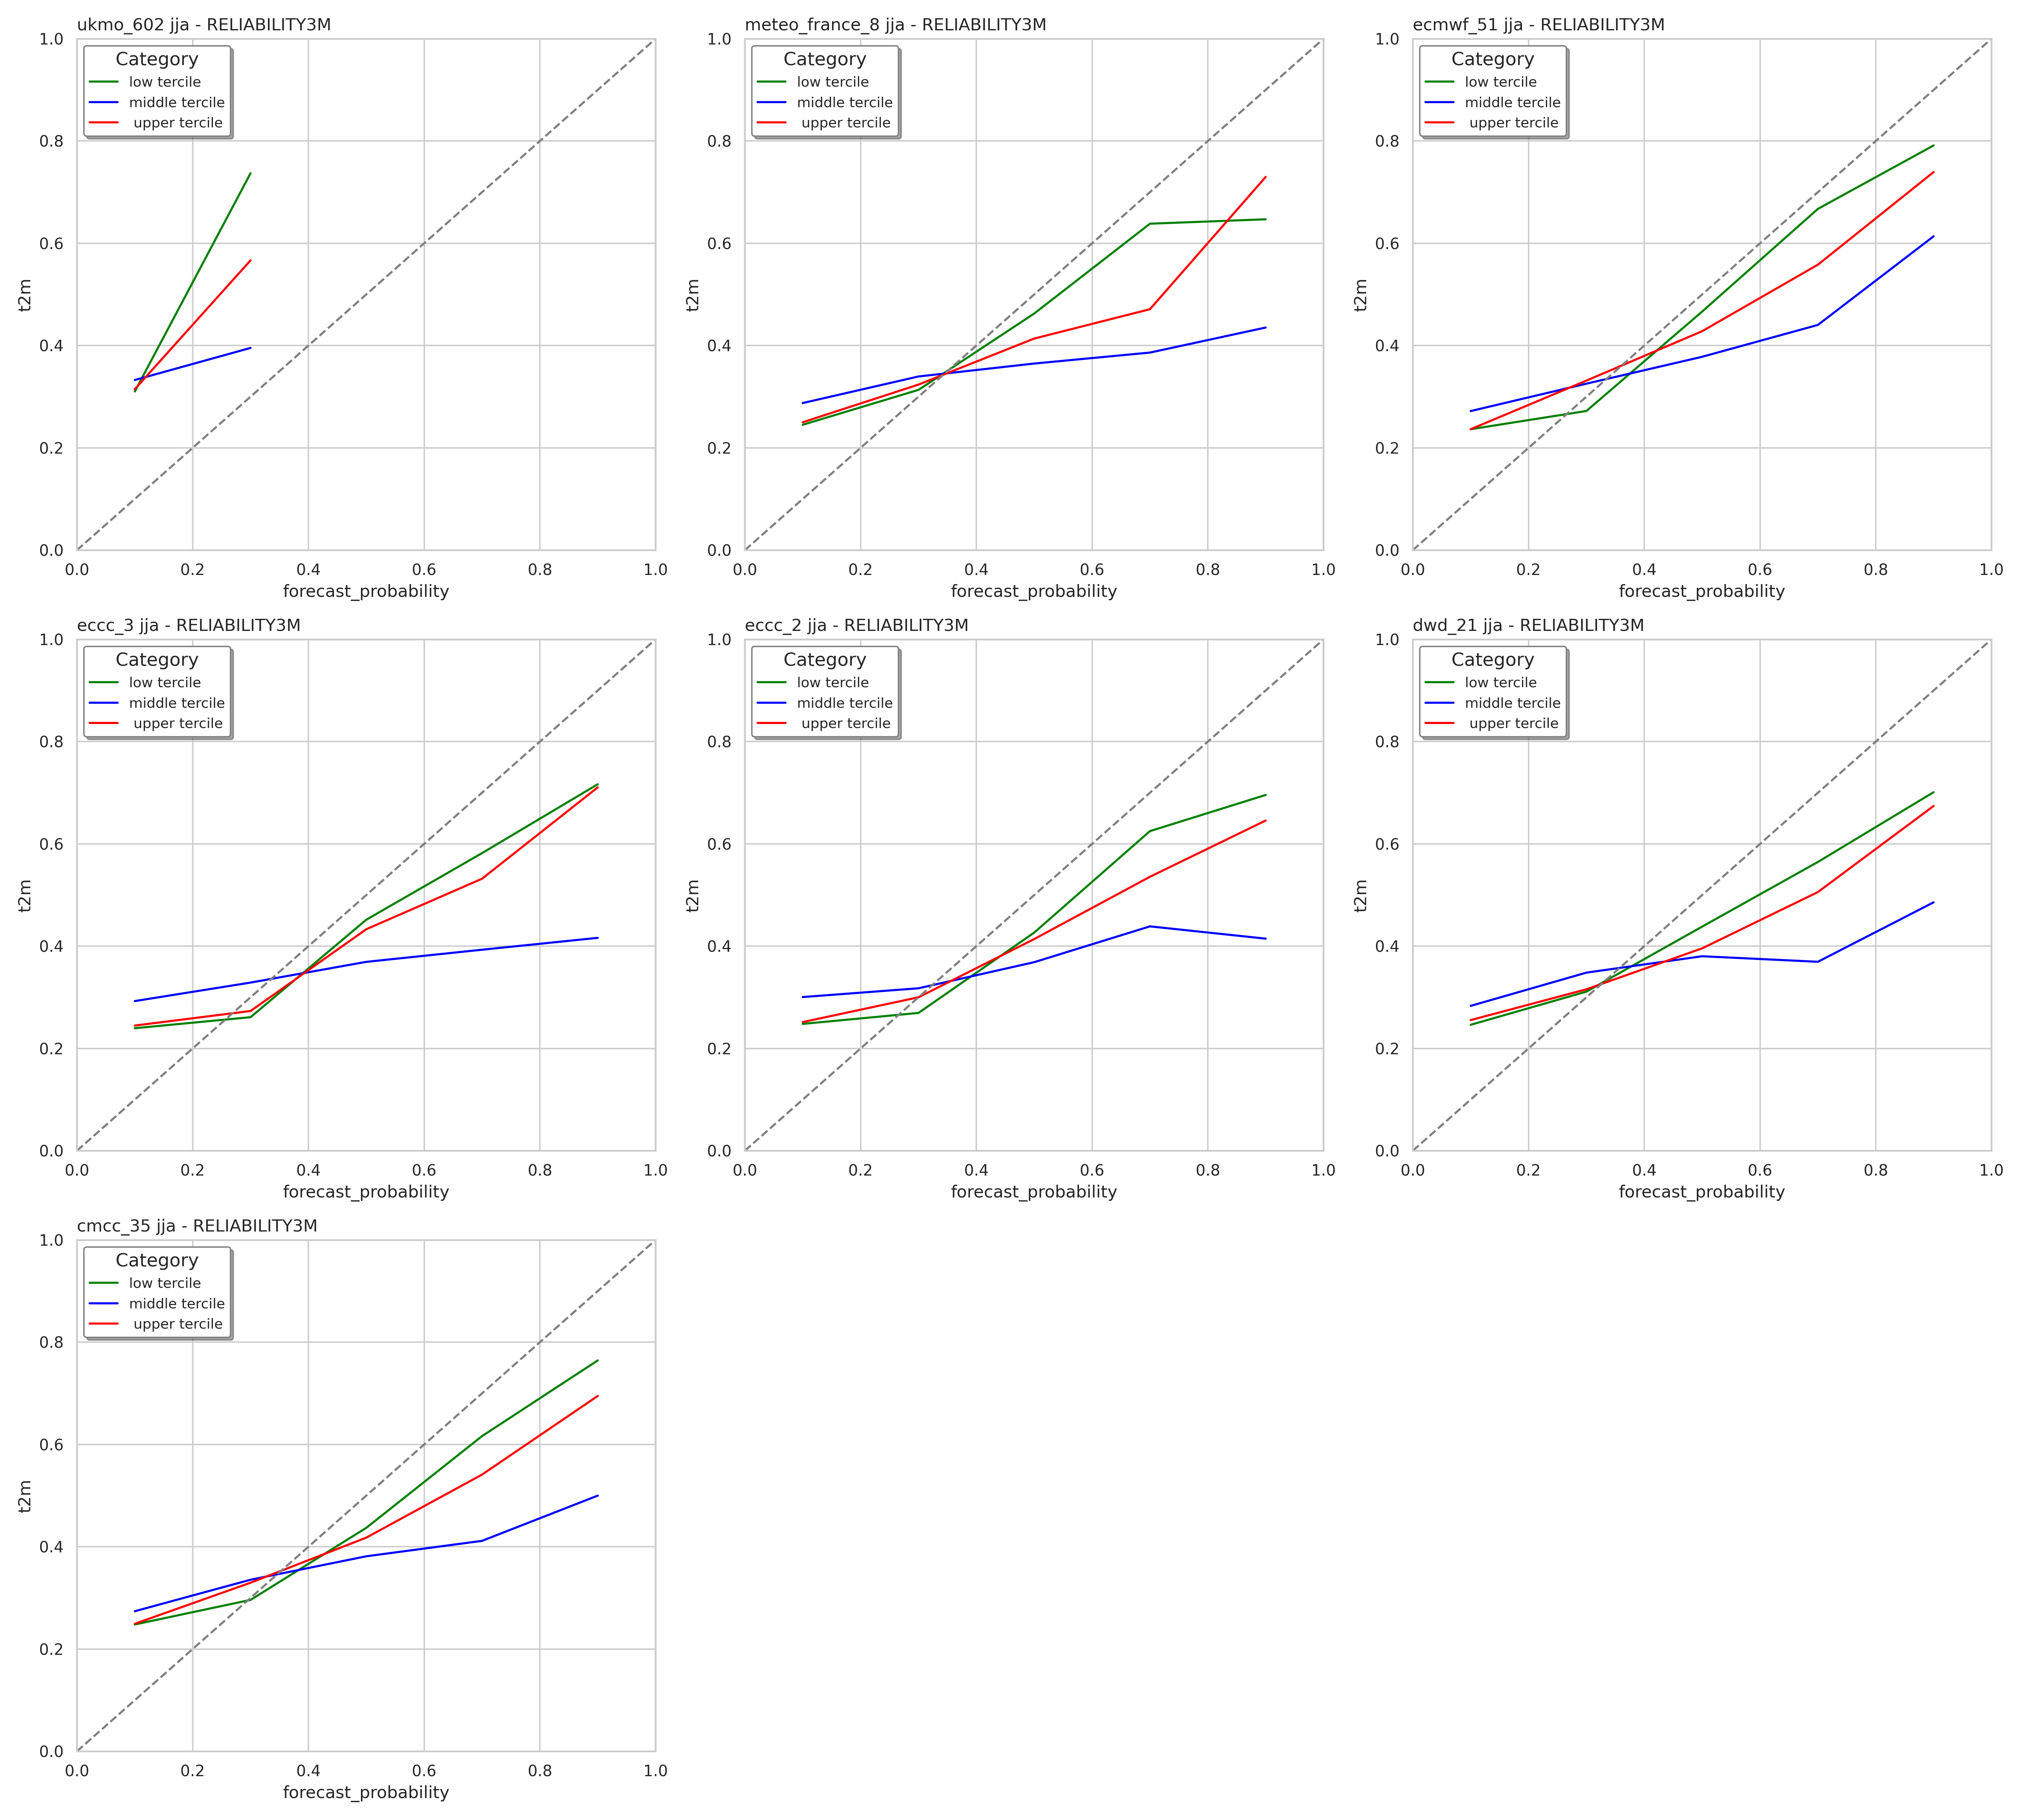
\includegraphics[scale=0.3]{rela_graphe.png}
\caption{The 3-month rolling mean for Reliability   . \textbf{\textit{Reliability is better in cases where the graphs are closer to the 45-degree line}}}
\end{figure}
for the 3-months rolling mean, the ECMWF has the best performance in reliability. The other centers have similar moderate performance, but the ukmo has poor reliability.







\subsubsection{The ranked probability score (RPS)}

The Ranked Probability Score (RPS) is a performance metric used in probabilistic forecasting to assess how well the predicted probability distribution matches the observed outcome distribution. It is particularly useful when there are multiple categories (e.g., terciles such as lower, middle, and upper) and is commonly applied in fields such as meteorology, climatology, and economics.

$$RPS=\frac{1}{n(m-1)}\sum\limits_{i=1}^{n} \sum\limits_{k=1}^{m-1} \left(\sum\limits_{j=1}^{k}(y_{j,i} - p_{j,i})\right)^2  $$

where : 

\begin{itemize}
	\item n is the number of forecasts.
	\item m is the number of categories.
	\item $y_{j,i}$ is 1 if the $i^th$ observation was in category j, and is 0 otherwise.
	\item $p_{j,i}$ is the $i^th$ forecast probability for category j
\end{itemize}

The score is the average squared “error” in the cumulative
probabilistic forecasts, and it ranges between 0\% for perfect forecasts (a probability of 100\%
was assigned to the observed category on each forecast) to a maximum of 100\% that can only
be achieved if all the observations are in the outermost categories, and if the forecasts are
perfectly bad (a probability of 100\% was assigned to the opposite outermost category to that
observed).


\begin{figure}[H]
    \centering
    \includegraphics[scale=0.25]{rps_T2M_ PERIOD.png}
    \caption{The Heatmap of  RPS Score on MENA region for T2M    . \textbf{\textit{(0 means perfect RPS)}}}
\end{figure}

In the figure above, all centers demonstrate similar performance, except for UKMO, which shows noticeably lower performance.




\subsubsection{Relative operating characteristics}
The ROC\footnote{wmo guidance verification} can be used in forecast verification to measure \textbf{\textit{the ability of the forecasts to distinguish an event from a non-event}}. For seasonal forecasts with three or more categories, the first
problem is to define the “event”. One of the categories must be selected as the current category
of interest, and an occurrence of this category is known as an event. An observation in any of
the other categories is defined as a non-event and no distinction is made as to which of these
two categories does occur. So, for example, if below normal is selected as the event, normal
and above normal are treated equally as non-events.

the score indicates the probability of successfully
discriminating below-normal observations from normal and above-normal observations. It
indicates how often the forecast probability for below normal is higher when below normal
actually does occur compared to when either normal or above normal occurs.


\begin{figure}[H]
    \centering
    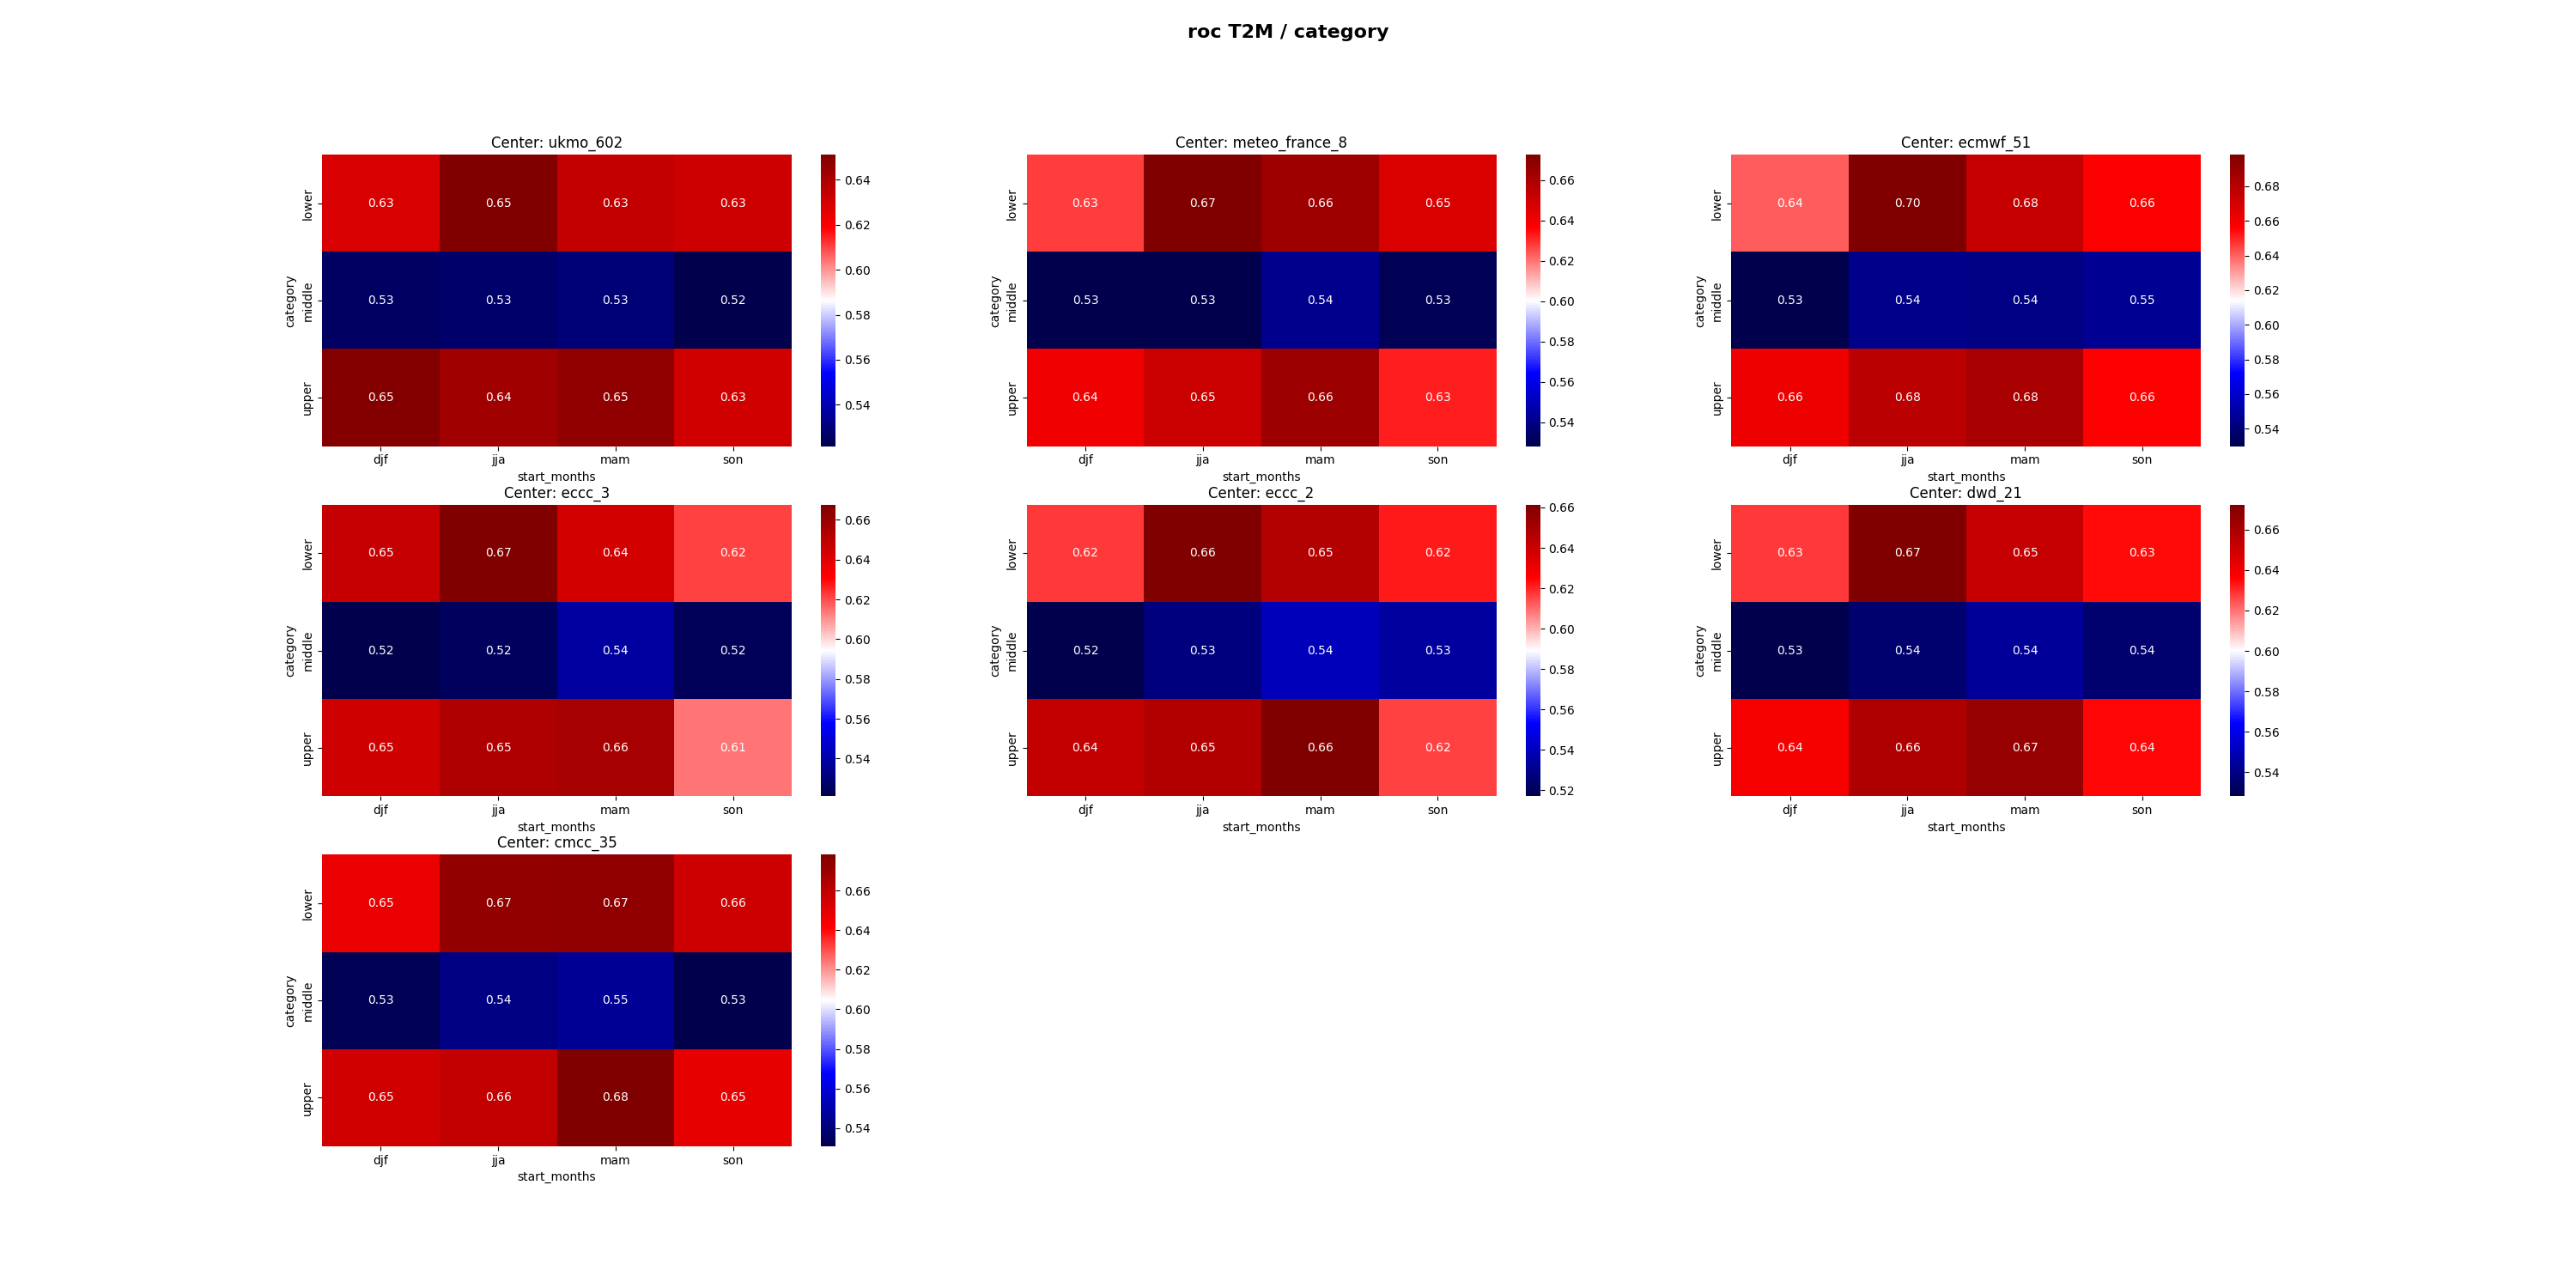
\includegraphics[scale=0.25]{roc_T2M_category.png}
    \caption{The Heatmap of ROC Score for each category  . \textbf{\textit{(1 means perfect ROC)}}}
\end{figure}

In the figure above, it is evident that all centers exhibit similar performance levels. However, the middle tercile consistently achieves the lowest score.
\begin{figure}[H]
    \centering
    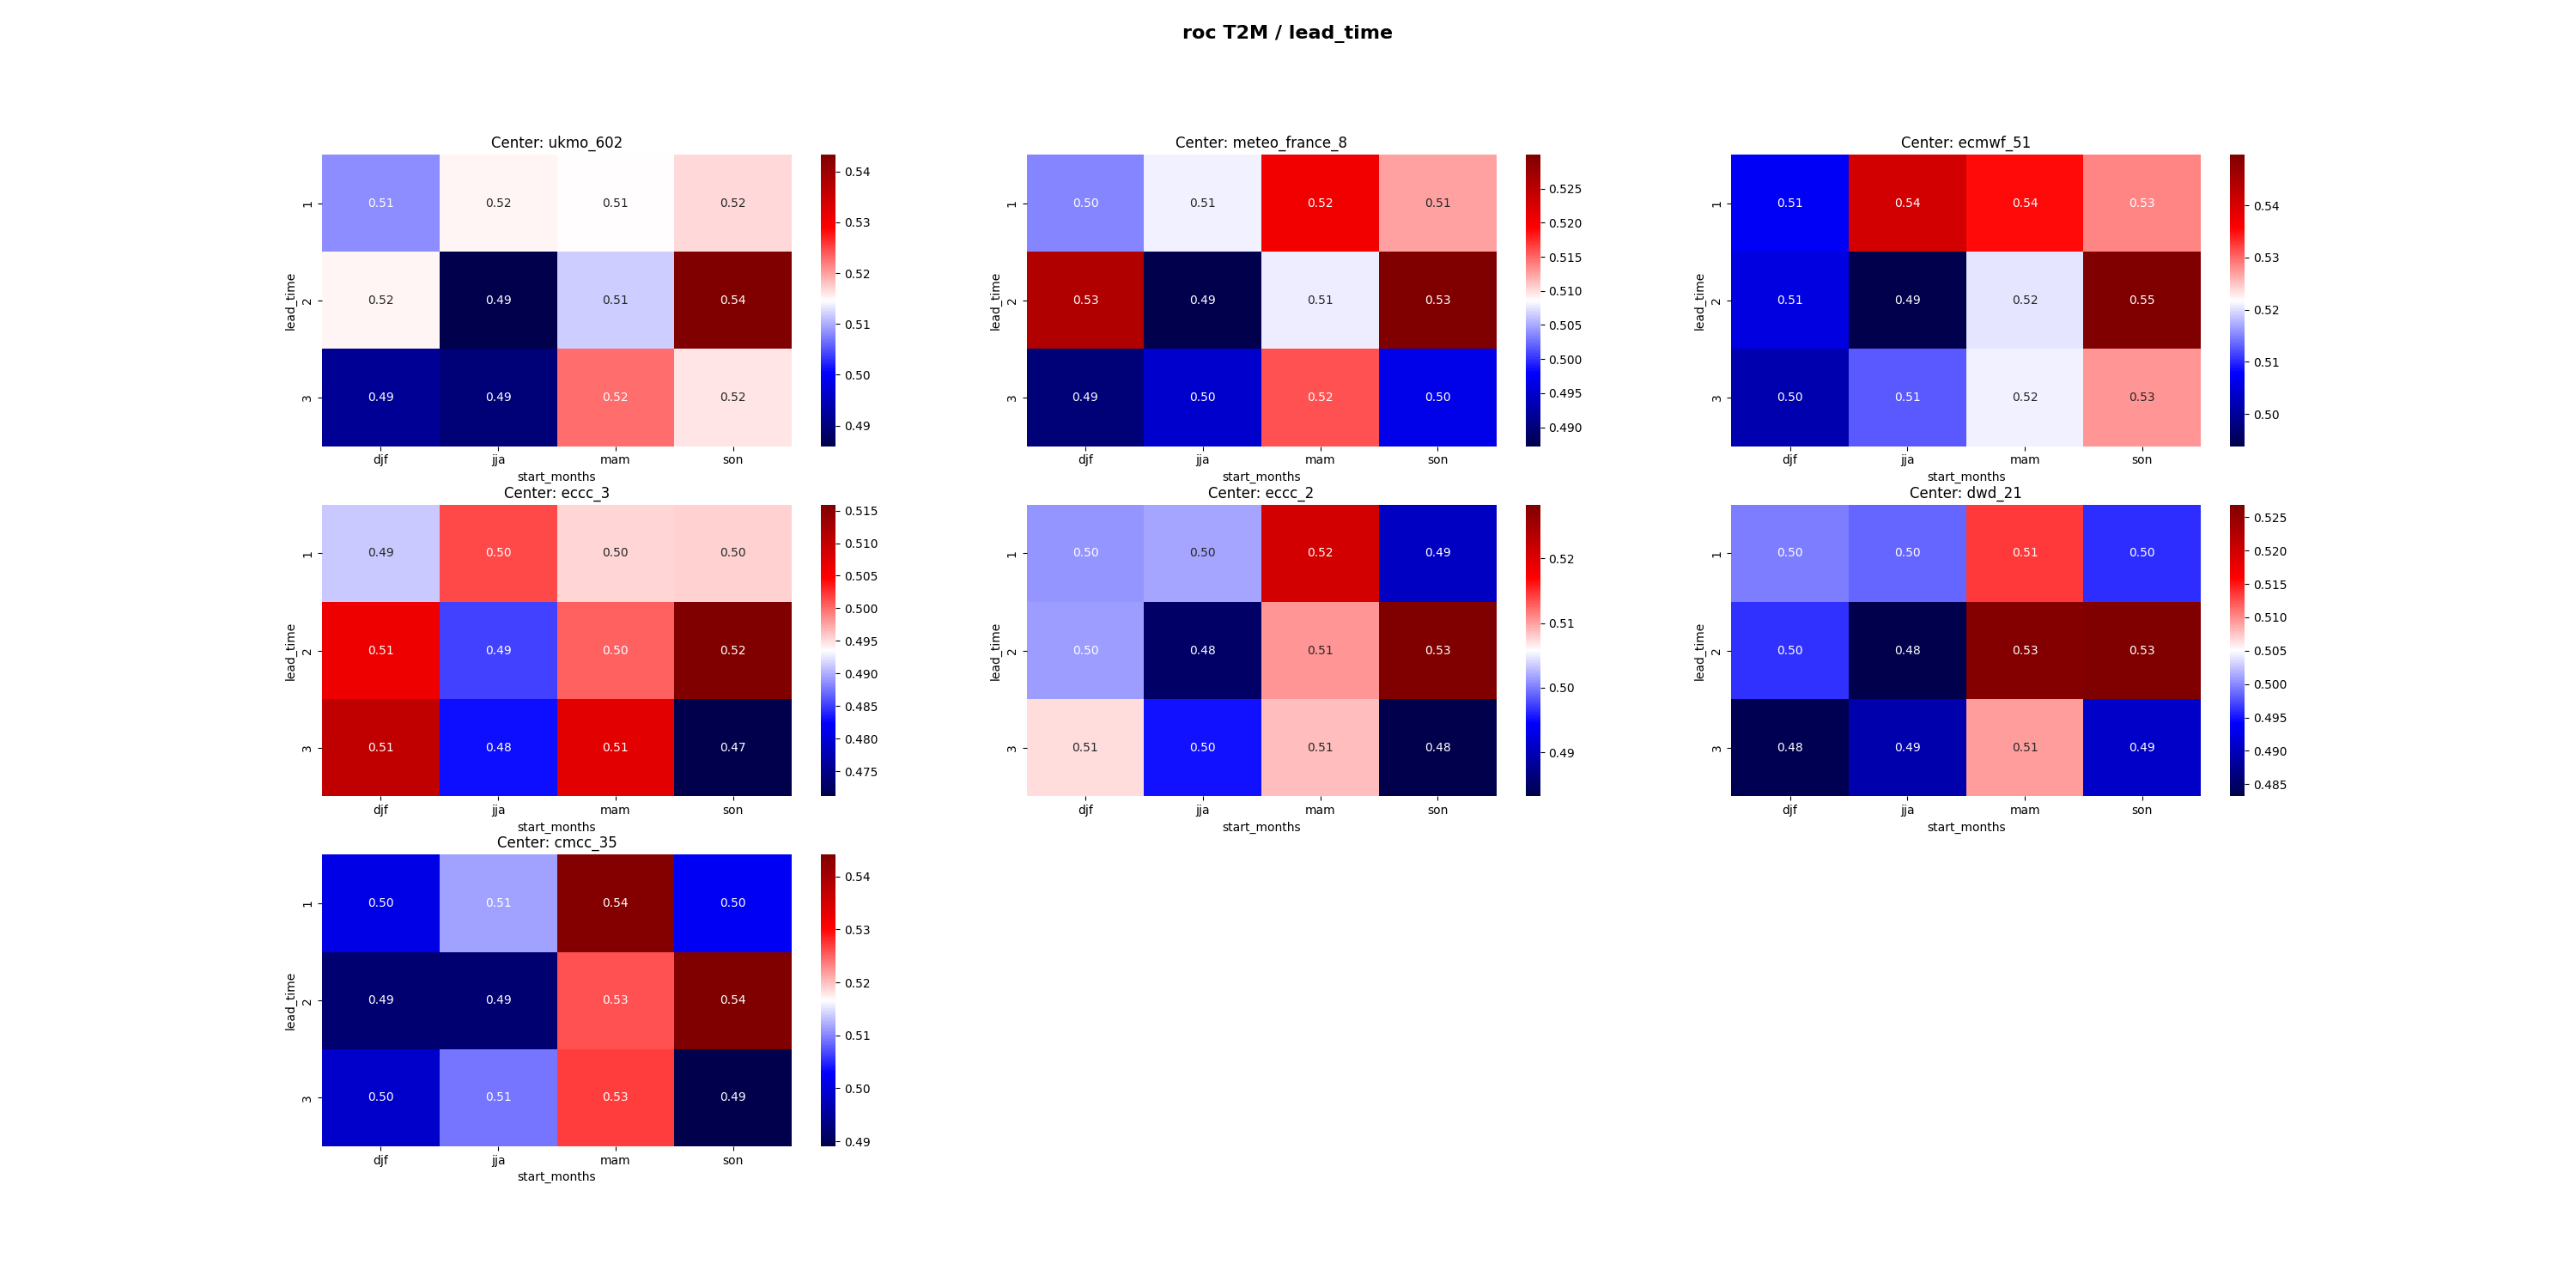
\includegraphics[scale=0.25]{roc_T2M_lead_time.png}
    \caption{The Heatmap of ROC Score for lead-times. \textbf{\textit{(1 means perfect ROC)}}}
\end{figure}


\begin{figure}[H]
    \centering
    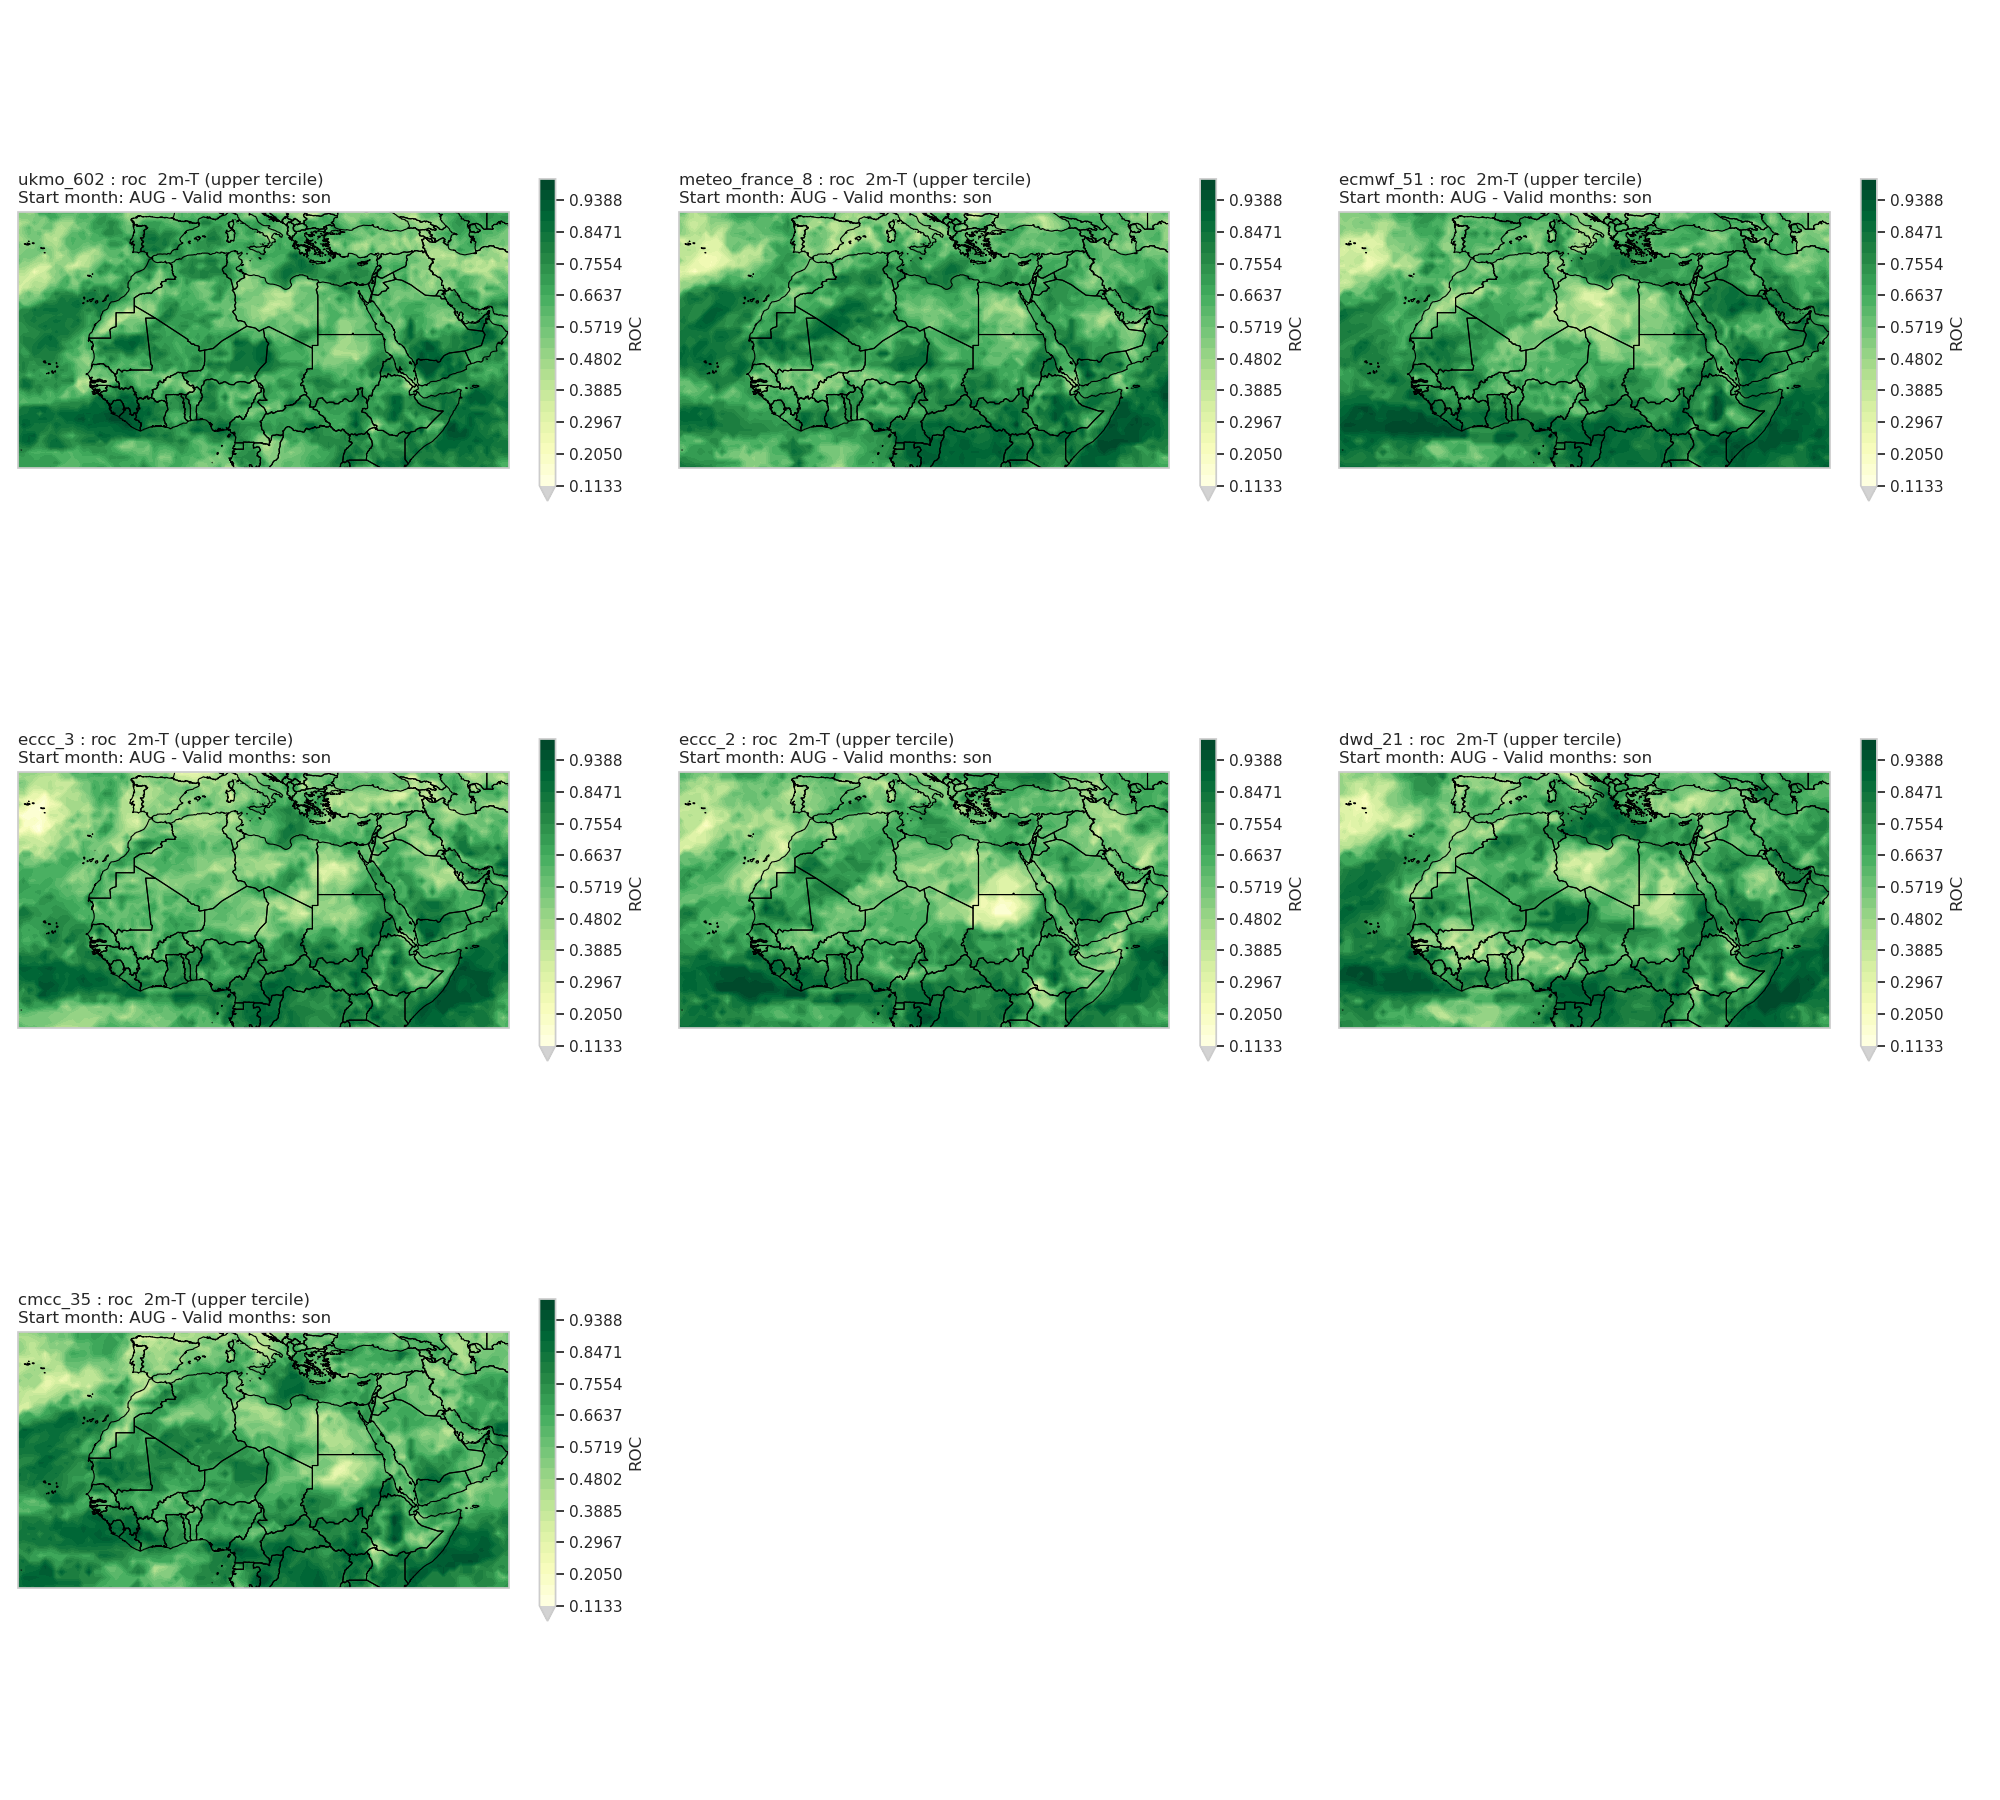
\includegraphics[scale=0.3]{ROC_UPPER_SON.png}
    \caption{The ROC Score Upper tercile SON    . \textbf{\textit{(1 means perfect ROC)}}}
\end{figure}


\subsubsection{Relative operating characteristics Skill Score}
The Relative Operating Characteristic Skill Score (ROCSS) is a measure used in forecast verification to assess the ability of probabilistic forecasts to discriminate between events and non-events. It builds on the Relative Operating Characteristic (ROC) curve, which plots the hit rate (true positive rate) against the false alarm rate (false positive rate) at various forecast probability thresholds.

\begin{itemize}
	\item The ROC curve evaluates the discrimination capability of a forecast, i.e., how well the forecast can separate occurrences of an event (e.g., below-normal temperature) from non-events (e.g., normal or above-normal temperature).
	\item The ROC Skill Score quantifies the area under the ROC curve (AUC) and compares it to a no-skill forecast.
\end{itemize}

	$$ROCSS=\frac{AUC-AUC_{no-skill}}{1-AUC_{no-skill}}$$
where:
\begin{itemize}
	\item $AUC$ : Area Under the ROC Curve for the forecast being evaluated.
	\item $AUC_{no-skill}$ : Area Under the Curve for a no-skill forecast 0.5 for our case.
\end{itemize}

Interpretation of ROCSS:
\begin{itemize}
	\item 1: Perfect discrimination ability.
	\item 0: No skill (forecast performs no better than random guessing).
	\item Negative values: Forecast performs worse than random guessing.
\end{itemize}
	

In the figure above, it is evident that the ECMWF exhibit the best performance for all terciles and periods. HOwever, we should notice that the performance is very bad for the middle tercile in all centers.

\begin{figure}[H]
    \centering
    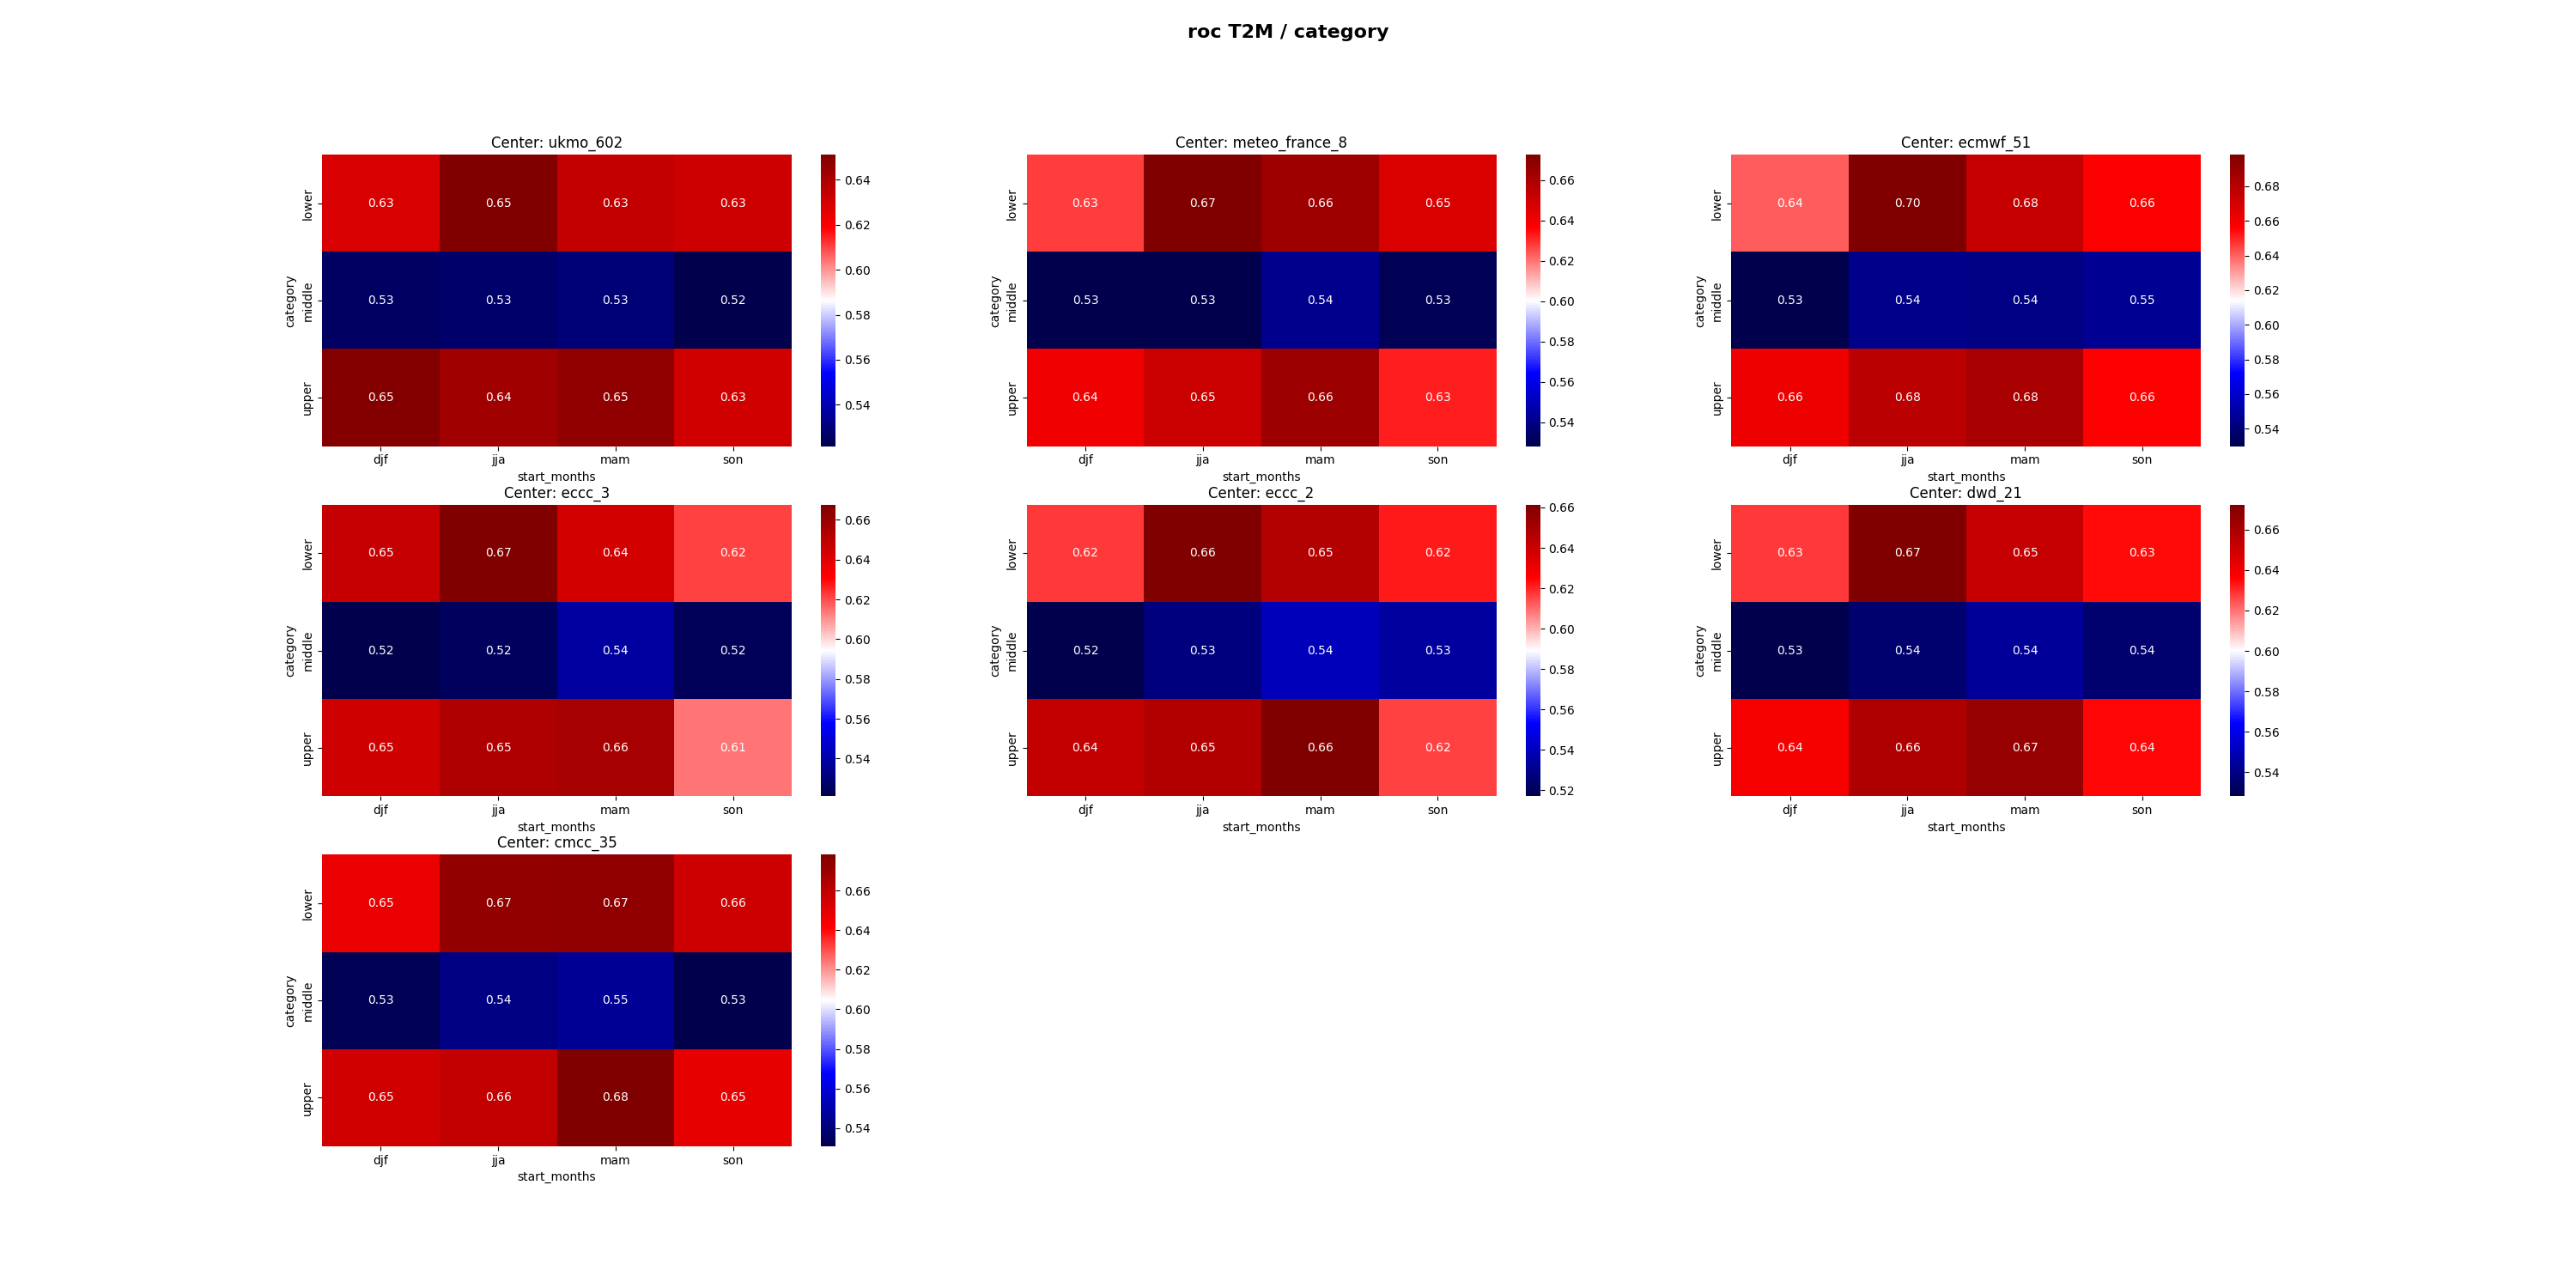
\includegraphics[scale=0.25]{roc_T2M_category.png}
    \caption{The ROCSS Score for each category  . \textbf{\textit{(1 means perfect ROCSS)}}}
\end{figure}


\begin{figure}[H]
    \centering
    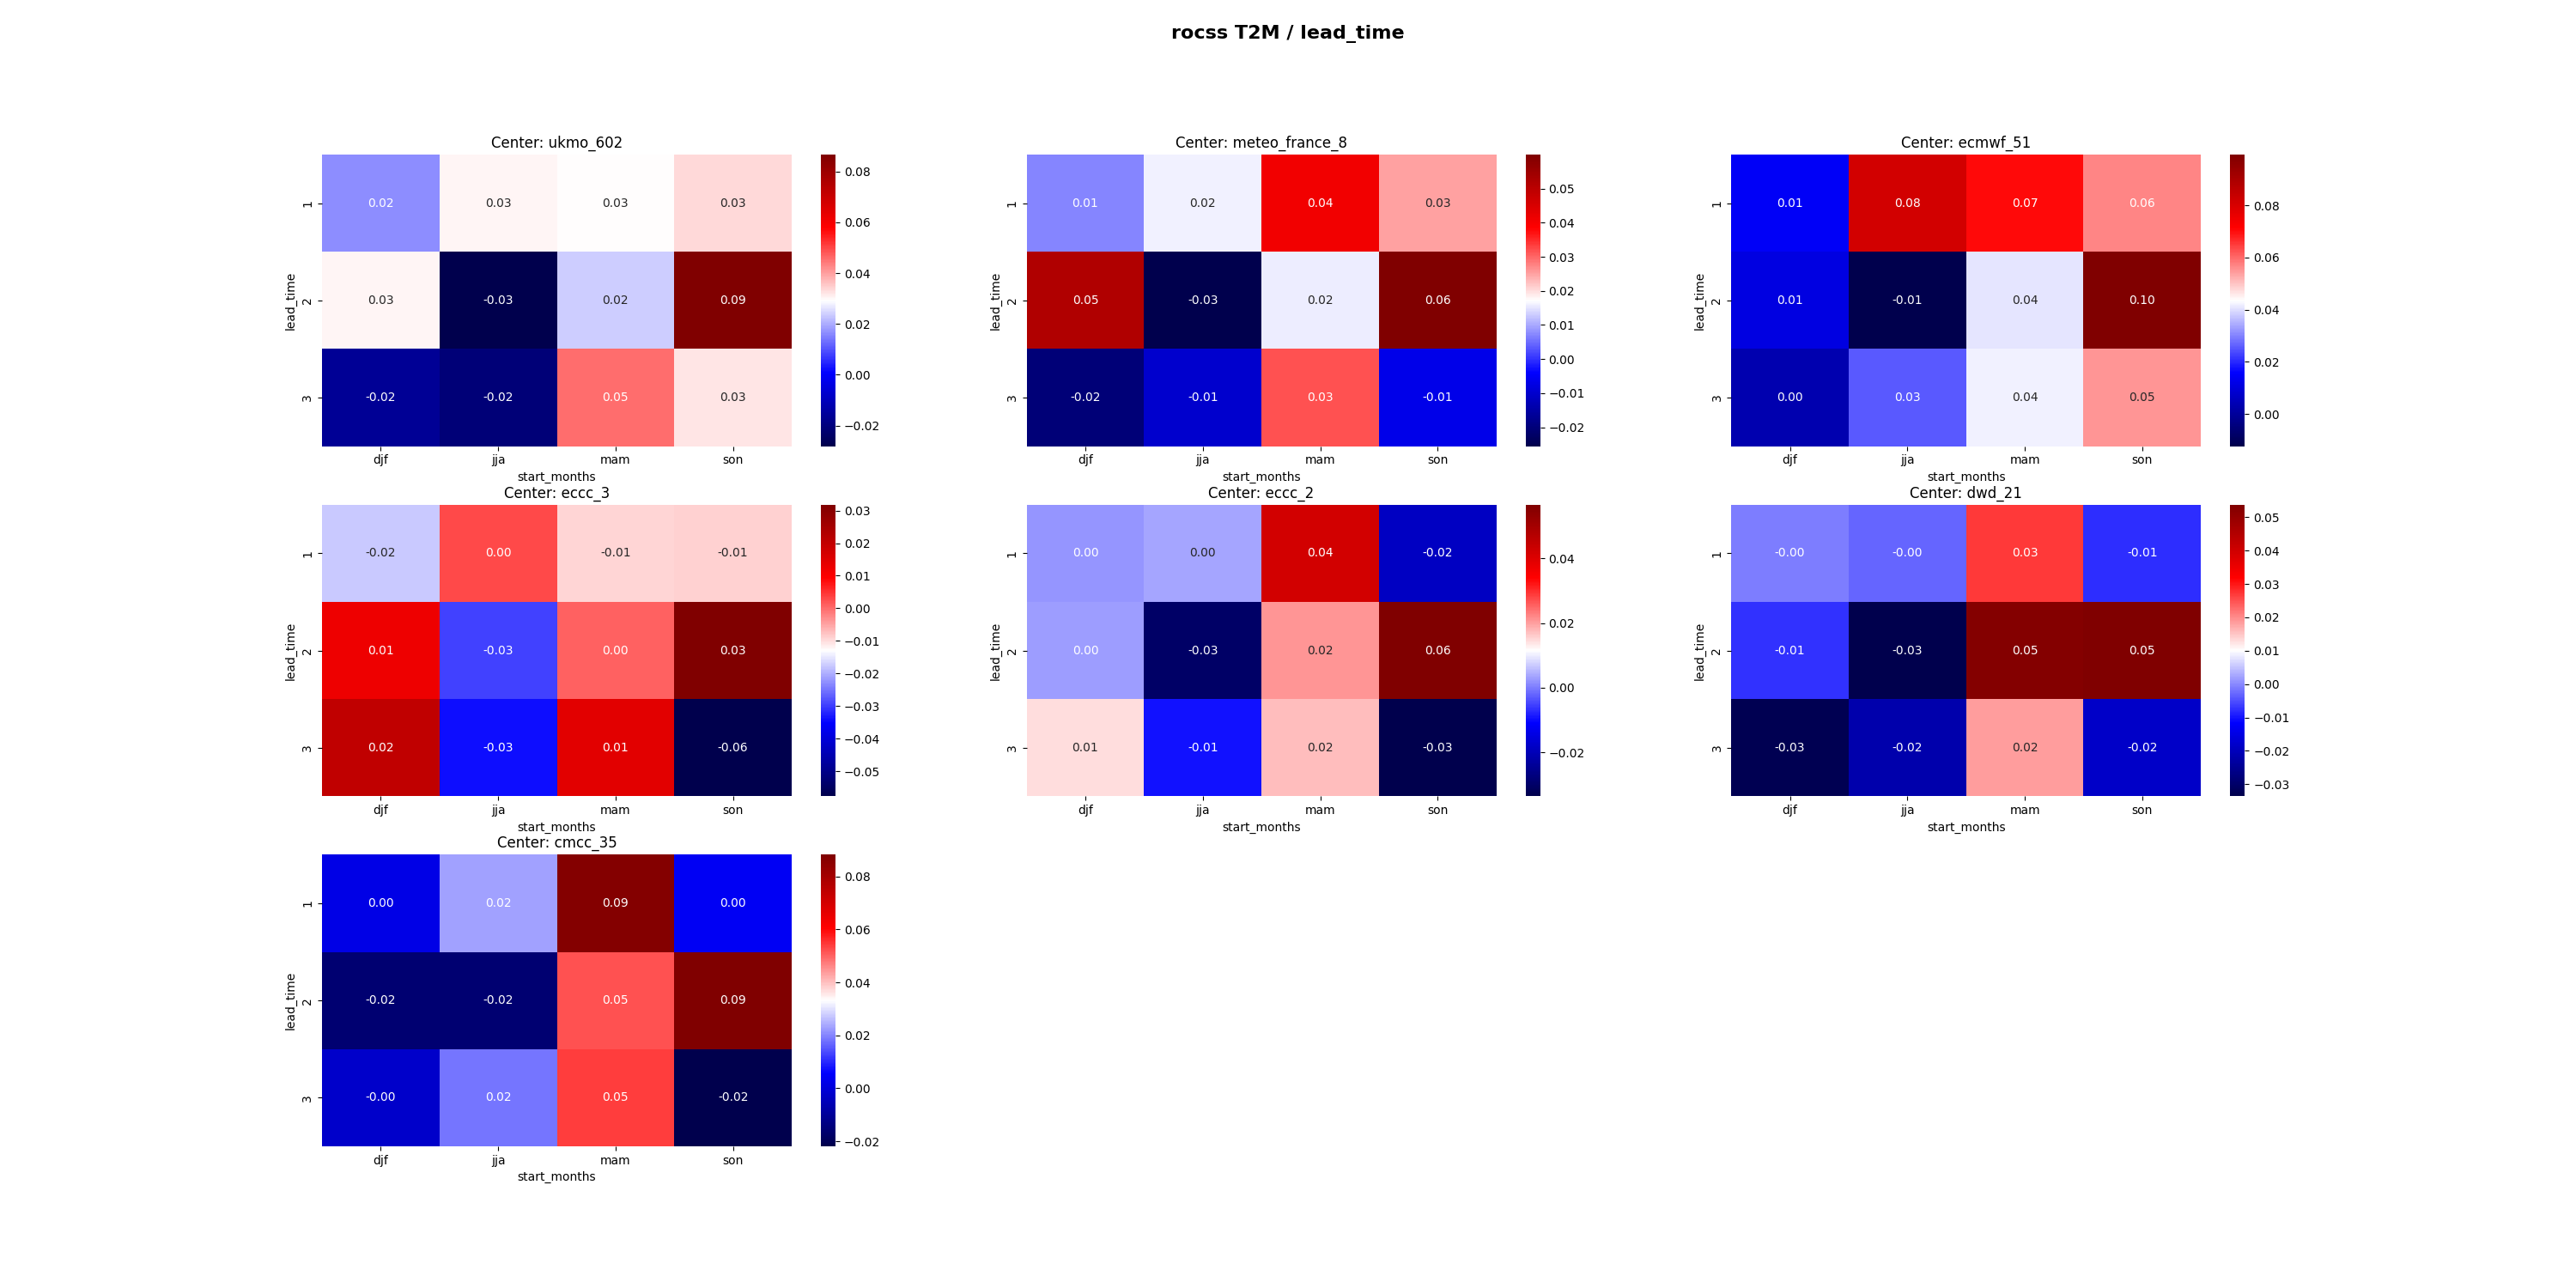
\includegraphics[scale=0.25]{rocss_T2M_lead_time.png}
    \caption{The average of  ROCSS Score on all categories    . \textbf{\textit{(1 means perfect ROCSS)}}}
\end{figure}


\begin{figure}[H]
    \centering
    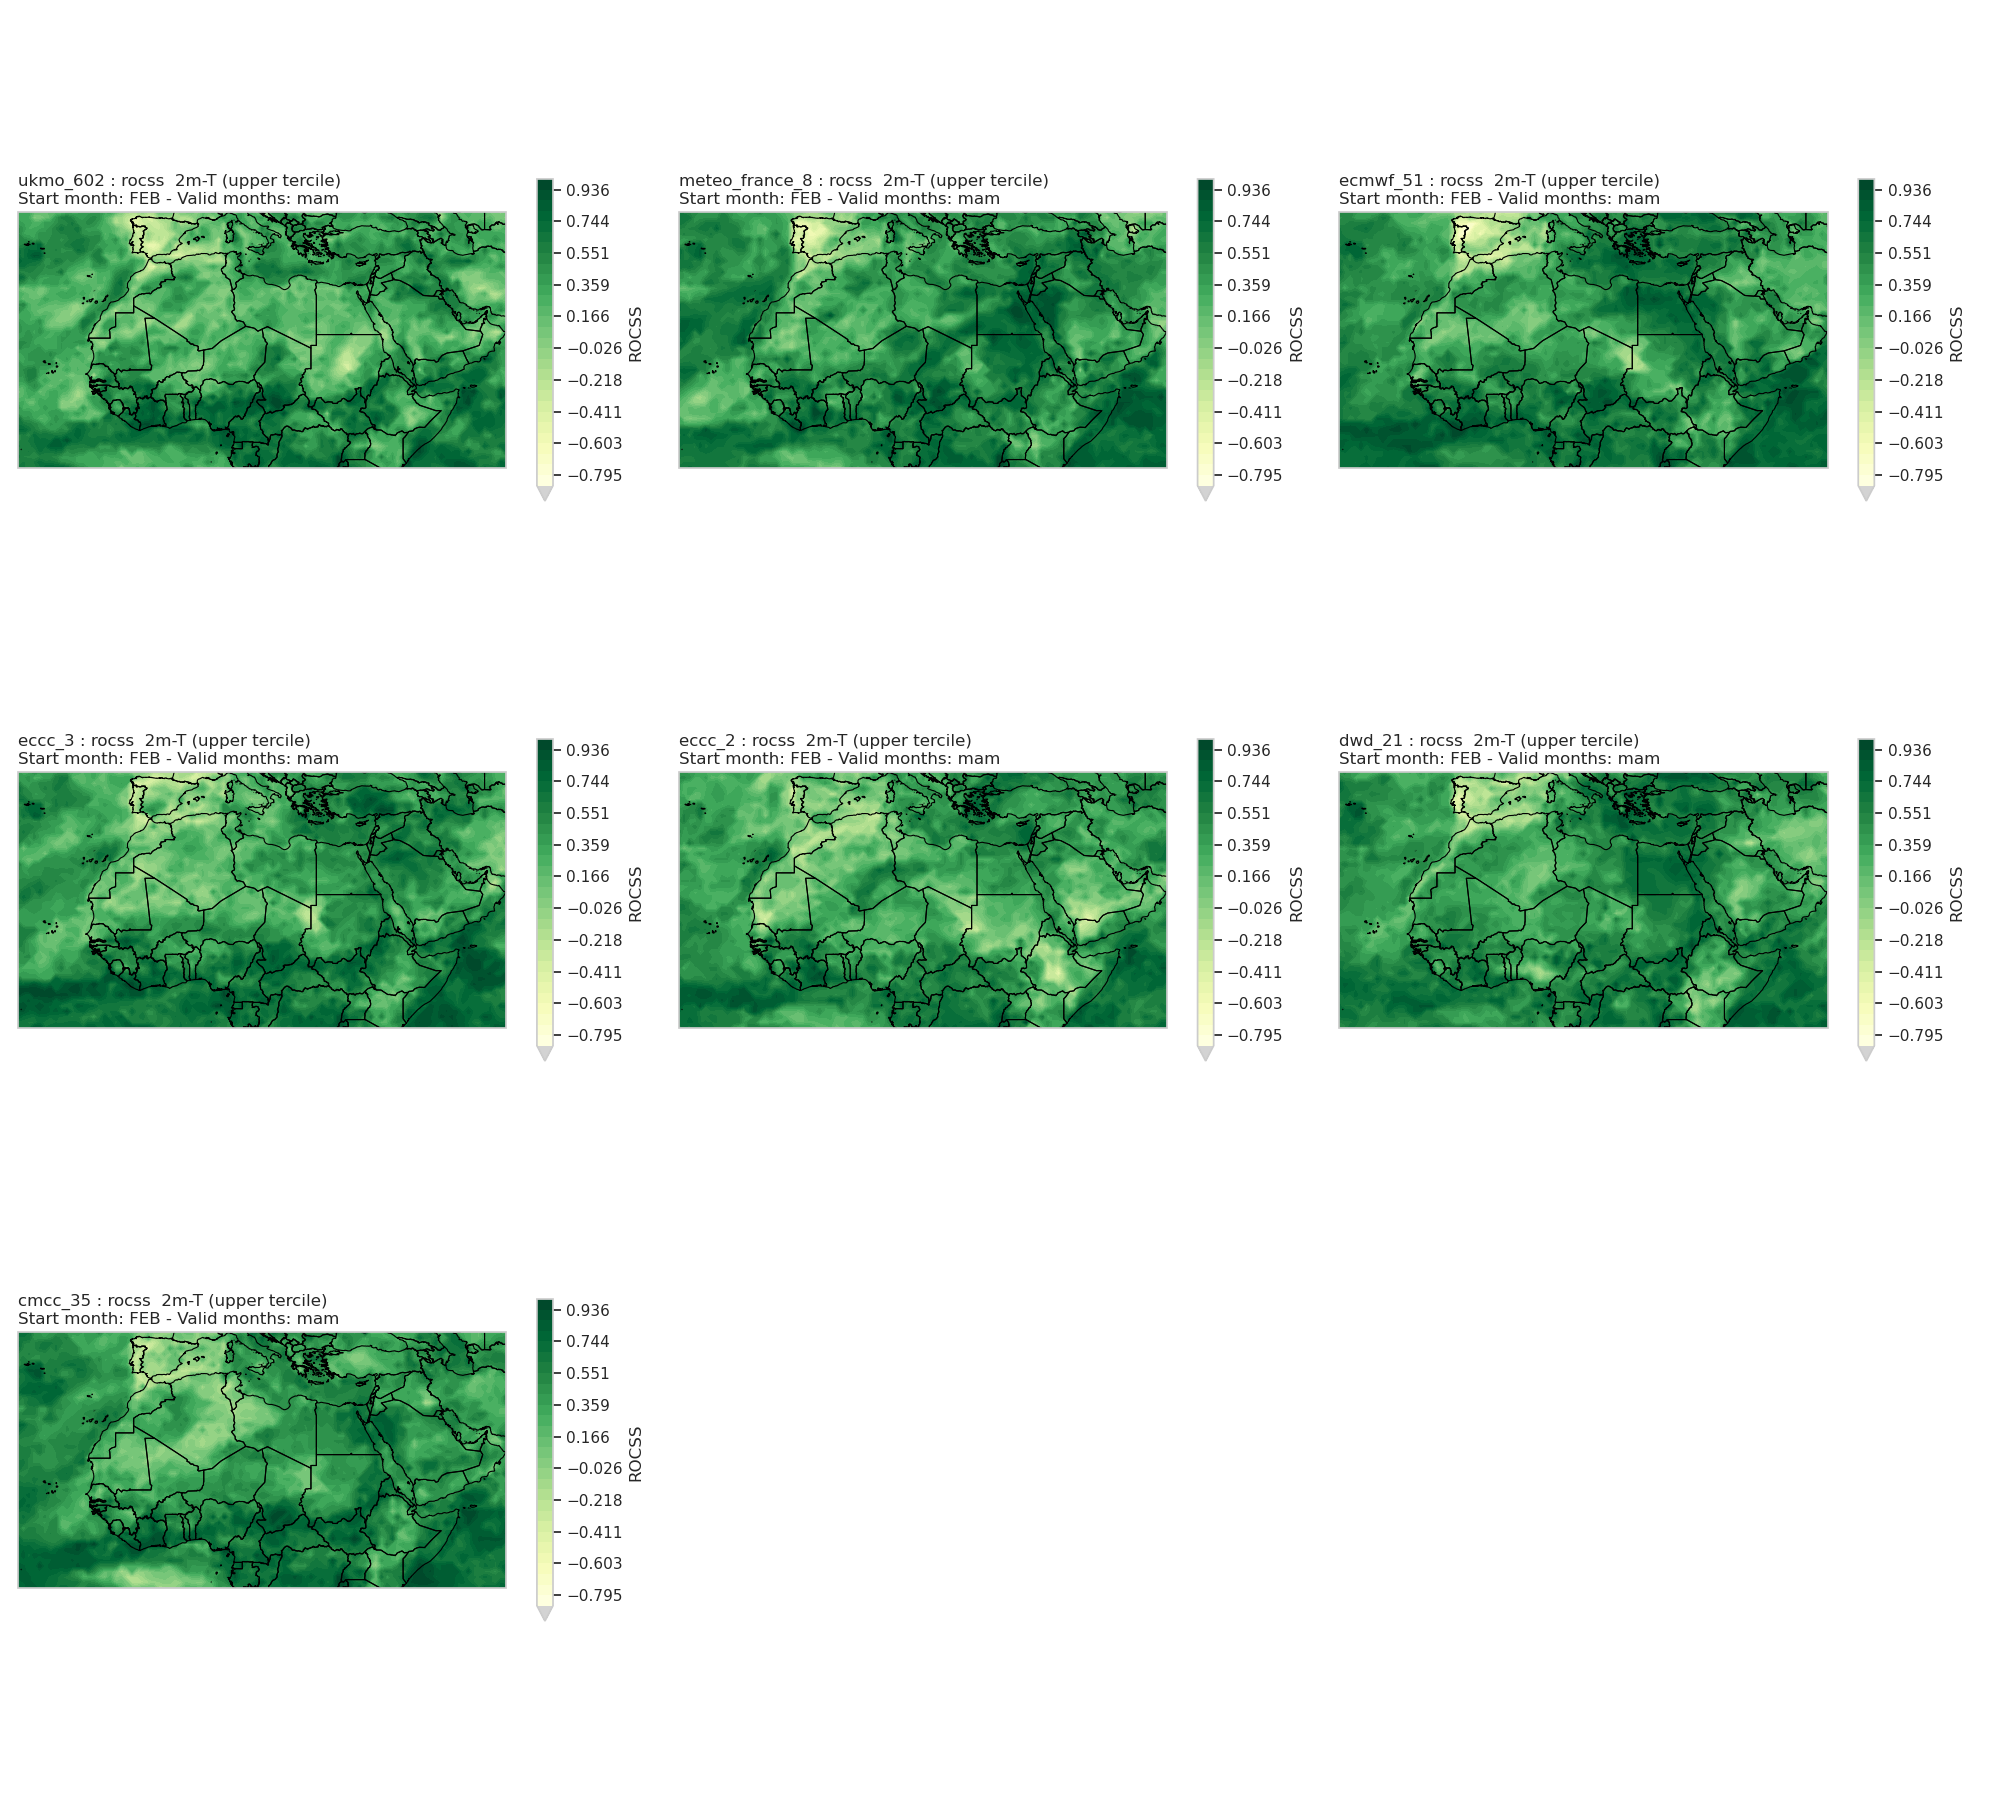
\includegraphics[scale=0.3]{ROCSS_MAM_UPPER.png}
    \caption{The ROC Skill Score Upper tercile MAM    . \textbf{\textit{(1 means perfect ROC)}}}
\end{figure}








\subsubsection{summary}
\begin{table}[h!]
\centering
\begin{tabularx}{\textwidth}{@{}p{2.5cm}p{4cm}p{4cm}p{2.5cm}p{3cm}@{}}
\toprule
\textbf{Metric}       & \textbf{Focus}                                    & \textbf{What it Measures}                         & \textbf{Dependent on Observed Outcomes?} & \textbf{Visualization/Tools}             \\ \midrule
\textbf{Reliability}   & Probabilities match observed frequencies          & Calibration of probabilities                      & Yes                                      & Reliability diagram                      \\
\textbf{Discrimination} & Differentiating between outcomes                 & Ability to distinguish events from non-events    & Yes                                      & ROC curve, AUC                           \\
\textbf{Sharpness}     & Boldness of probabilities (away from average)     & Confidence of the forecast                        & No                                       & Histogram of forecast probabilities      \\
\textbf{Resolution}    & Informativeness and variability of forecast       & Ability to provide specific, useful info         & Yes                                      & Brier Score decomposition                \\ \bottomrule
\end{tabularx}
\caption{Key differences between reliability, discrimination, sharpness, and resolution in seasonal forecasting.}
\label{tab:forecast_metrics}
\end{table}

\newpage
\thispagestyle{empty}
\mbox{}  % Include content from SCORES.tex file
\clearpage
\listoffigures
\clearpage
\listoftables

\end{document}
